% One page with Figure 1 and its caption, on the page and text block of the
% Bioinformatics template used in ../vepyr-overleaf (oup-authoring-template,
% options contemporary,large): paper 209.80 x 275.84 mm, text block 488.5 pt x
% 63 lines of 10.5 pt, caption in 6 bp on 9 pt with a bold "Fig. 1." label and
% 13 pt above it. The class itself needs packages missing from this TeX
% installation, so its dimensions are reproduced here. The figure is the
% TikZ picture of build_tikz.py. The grey frame marks
% the text block; the line below it reports the space left.
%
%   pdflatex figure1-page.tex
\documentclass{article}
\usepackage{fix-cm}
\usepackage[T1]{fontenc}
\usepackage{lmodern}
\usepackage[paperwidth=209.80mm, paperheight=275.84mm, textwidth=488.5pt,
  textheight=661.5pt, left=54.6pt, top=56.68pt, headheight=0pt, headsep=0pt,
  footskip=16pt]{geometry}
\usepackage{graphicx}
\usepackage{xcolor}
\usepackage{colortbl}
\usepackage{array}
\usepackage{booktabs}
\usepackage{tikz}
\usetikzlibrary{arrows.meta}
\usepackage{eso-pic}
\pagestyle{empty}

\makeatletter
\AddToShipoutPictureBG{%
  \AtTextLowerLeft{\color{black!25}\linethickness{0.3pt}%
    \put(0,0){\framebox(\strip@pt\textwidth,\strip@pt\textheight){}}}}
\makeatother

\newsavebox\figbox
% Panel A of Figure 1, generated by build_tikz.py from ../tool-comparison.
\definecolor{muted}{HTML}{57606A}
\definecolor{hl}{HTML}{EAF2FB}
\definecolor{todo}{HTML}{CF222E}
\newsavebox\figonetablebox
\newcommand{\figonetable}{{%
\sffamily\fontsize{7}{8.2}\selectfont
\setlength{\tabcolsep}{0.8mm}\renewcommand{\arraystretch}{1.12}%
\aboverulesep=0.6ex \belowrulesep=0.6ex
\heavyrulewidth=0.6pt \lightrulewidth=0.35pt
\sbox\figonetablebox{\begin{tabular}{@{}>{\raggedright\arraybackslash}p{5.40cm}>{\raggedright\arraybackslash}p{7.00cm}>{\raggedright\arraybackslash}p{7.00cm}>{\raggedright\arraybackslash}p{7.00cm}>{\columncolor{hl}\raggedright\arraybackslash}p{7.00cm}@{}}
\toprule
 & Ensembl VEP\newline{\fontsize{5.8}{6.6}\selectfont\color{muted}116.0\enspace\texttt{57ea5c5}} & fastVEP\newline{\fontsize{5.8}{6.6}\selectfont\color{muted}0.4.0+6\enspace\texttt{5d8004a}} & vep-rs\newline{\fontsize{5.8}{6.6}\selectfont\color{muted}0.4.0\enspace\texttt{f642723}} & \textbf{vepyr}\newline{\fontsize{5.8}{6.6}\selectfont\color{muted}0.10.0\enspace\texttt{3f21520}} \\
\midrule
\textcolor{muted}{Language} & Perl & Rust & Rust & Rust, Python \\
\textcolor{muted}{Parallelism} & processes & threads & threads & threads \\
\textcolor{muted}{Cache format} & Storable, gzip per 1-Mb region & bincode + zstd (transcripts), OSAv2 (annotations) & JSON, gzip optional & Parquet, ZSTD (core and plugins) \\
\textcolor{muted}{Fields filled\textsuperscript{a}} & 80/80 & \ensuremath{\leq}37/80 & \ensuremath{\leq}71/80 (34/80)\textsuperscript{b} & \textbf{80/80} \\
\textcolor{muted}{Transcript sets} & Ensembl, RefSeq, merged & Ensembl, RefSeq, merged\textsuperscript{c} & Ensembl, RefSeq, merged\textsuperscript{d} & Ensembl, RefSeq, merged \\
\textcolor{muted}{Declared variant classes} & SNV, indel, SV & SNV, indel, SV\textsuperscript{e} & SNV, indel, SV\textsuperscript{e} & SNV, indel \\
\textcolor{muted}{External annotation sources} & yes & yes & yes & yes \\
\textcolor{muted}{Concordance (chr22, merged)} & reference & \textcolor{todo}{\textbf{TODO}} & \textcolor{todo}{\textbf{TODO}} & \textcolor{todo}{\textbf{TODO}} \\
\textcolor{muted}{Interfaces} & CLI, web, REST & CLI, web, REST & CLI & Python API, SQL, CLI \\
\textcolor{muted}{Evaluation} & streaming & streaming & streaming & \textbf{lazy, \mbox{pushdown}} \\
\textcolor{muted}{Output} & VCF, tab, JSON & VCF, tab, JSON & VCF, tab, JSON, Parquet & Polars DataFrame/\allowbreak LazyFrame, VCF \\
\bottomrule
\end{tabular}}%
\vbox{\copy\figonetablebox\vskip 3pt
\hsize=\wd\figonetablebox \parindent=0pt
{\fontsize{5.6}{6.8}\selectfont\color{muted}\raggedright
\textsuperscript{a}Of the 80 \texttt{CSQ} fields of VEP~116 \texttt{--everything} (Ensembl cache), those the tool can fill, counted from its source code and documentation. \textsuperscript{b}34/80 on the cache converted from VEP, used for all concordance results (no known variants, SIFT or PolyPhen). \textsuperscript{c}From Ensembl and RefSeq GFF3 files (merged: both, with \texttt{SOURCE}); RefSeq-specific fields are not written. \textsuperscript{d}Through a cache converted from the VEP RefSeq or merged cache; \texttt{SOURCE} and the RefSeq fields are not written. \textsuperscript{e}As declared by the authors; SV annotation not fully validated against VEP.\par}}}}

\newcommand{\everything}{\texttt{-{}-everything}}

\begin{document}
\sbox\figbox{\parbox[t]{\textwidth}{%
\noindent% Figure 1, generated by build_tikz.py from build_figure1_v2.py; do not edit by
% hand, change the builders and regenerate. Width: \textwidth of the
% Bioinformatics template (488.5 pt). Needs % Panel A of Figure 1, generated by build_tikz.py from ../tool-comparison.
\definecolor{muted}{HTML}{57606A}
\definecolor{hl}{HTML}{EAF2FB}
\definecolor{todo}{HTML}{CF222E}
\newsavebox\figonetablebox
\newcommand{\figonetable}{{%
\sffamily\fontsize{7}{8.2}\selectfont
\setlength{\tabcolsep}{0.8mm}\renewcommand{\arraystretch}{1.12}%
\aboverulesep=0.6ex \belowrulesep=0.6ex
\heavyrulewidth=0.6pt \lightrulewidth=0.35pt
\sbox\figonetablebox{\begin{tabular}{@{}>{\raggedright\arraybackslash}p{5.40cm}>{\raggedright\arraybackslash}p{7.00cm}>{\raggedright\arraybackslash}p{7.00cm}>{\raggedright\arraybackslash}p{7.00cm}>{\columncolor{hl}\raggedright\arraybackslash}p{7.00cm}@{}}
\toprule
 & Ensembl VEP\newline{\fontsize{5.8}{6.6}\selectfont\color{muted}116.0\enspace\texttt{57ea5c5}} & fastVEP\newline{\fontsize{5.8}{6.6}\selectfont\color{muted}0.4.0+6\enspace\texttt{5d8004a}} & vep-rs\newline{\fontsize{5.8}{6.6}\selectfont\color{muted}0.4.0\enspace\texttt{f642723}} & \textbf{vepyr}\newline{\fontsize{5.8}{6.6}\selectfont\color{muted}0.10.0\enspace\texttt{3f21520}} \\
\midrule
\textcolor{muted}{Language} & Perl & Rust & Rust & Rust, Python \\
\textcolor{muted}{Parallelism} & processes & threads & threads & threads \\
\textcolor{muted}{Cache format} & Storable, gzip per 1-Mb region & bincode + zstd (transcripts), OSAv2 (annotations) & JSON, gzip optional & Parquet, ZSTD (core and plugins) \\
\textcolor{muted}{Fields filled\textsuperscript{a}} & 80/80 & \ensuremath{\leq}37/80 & \ensuremath{\leq}71/80 (34/80)\textsuperscript{b} & \textbf{80/80} \\
\textcolor{muted}{Transcript sets} & Ensembl, RefSeq, merged & Ensembl, RefSeq, merged\textsuperscript{c} & Ensembl, RefSeq, merged\textsuperscript{d} & Ensembl, RefSeq, merged \\
\textcolor{muted}{Declared variant classes} & SNV, indel, SV & SNV, indel, SV\textsuperscript{e} & SNV, indel, SV\textsuperscript{e} & SNV, indel \\
\textcolor{muted}{External annotation sources} & yes & yes & yes & yes \\
\textcolor{muted}{Concordance (chr22, merged)} & reference & \textcolor{todo}{\textbf{TODO}} & \textcolor{todo}{\textbf{TODO}} & \textcolor{todo}{\textbf{TODO}} \\
\textcolor{muted}{Interfaces} & CLI, web, REST & CLI, web, REST & CLI & Python API, SQL, CLI \\
\textcolor{muted}{Evaluation} & streaming & streaming & streaming & \textbf{lazy, \mbox{pushdown}} \\
\textcolor{muted}{Output} & VCF, tab, JSON & VCF, tab, JSON & VCF, tab, JSON, Parquet & Polars DataFrame/\allowbreak LazyFrame, VCF \\
\bottomrule
\end{tabular}}%
\vbox{\copy\figonetablebox\vskip 3pt
\hsize=\wd\figonetablebox \parindent=0pt
{\fontsize{5.6}{6.8}\selectfont\color{muted}\raggedright
\textsuperscript{a}Of the 80 \texttt{CSQ} fields of VEP~116 \texttt{--everything} (Ensembl cache), those the tool can fill, counted from its source code and documentation. \textsuperscript{b}34/80 on the cache converted from VEP, used for all concordance results (no known variants, SIFT or PolyPhen). \textsuperscript{c}From Ensembl and RefSeq GFF3 files (merged: both, with \texttt{SOURCE}); RefSeq-specific fields are not written. \textsuperscript{d}Through a cache converted from the VEP RefSeq or merged cache; \texttt{SOURCE} and the RefSeq fields are not written. \textsuperscript{e}As declared by the authors; SV annotation not fully validated against VEP.\par}}}}
 first.
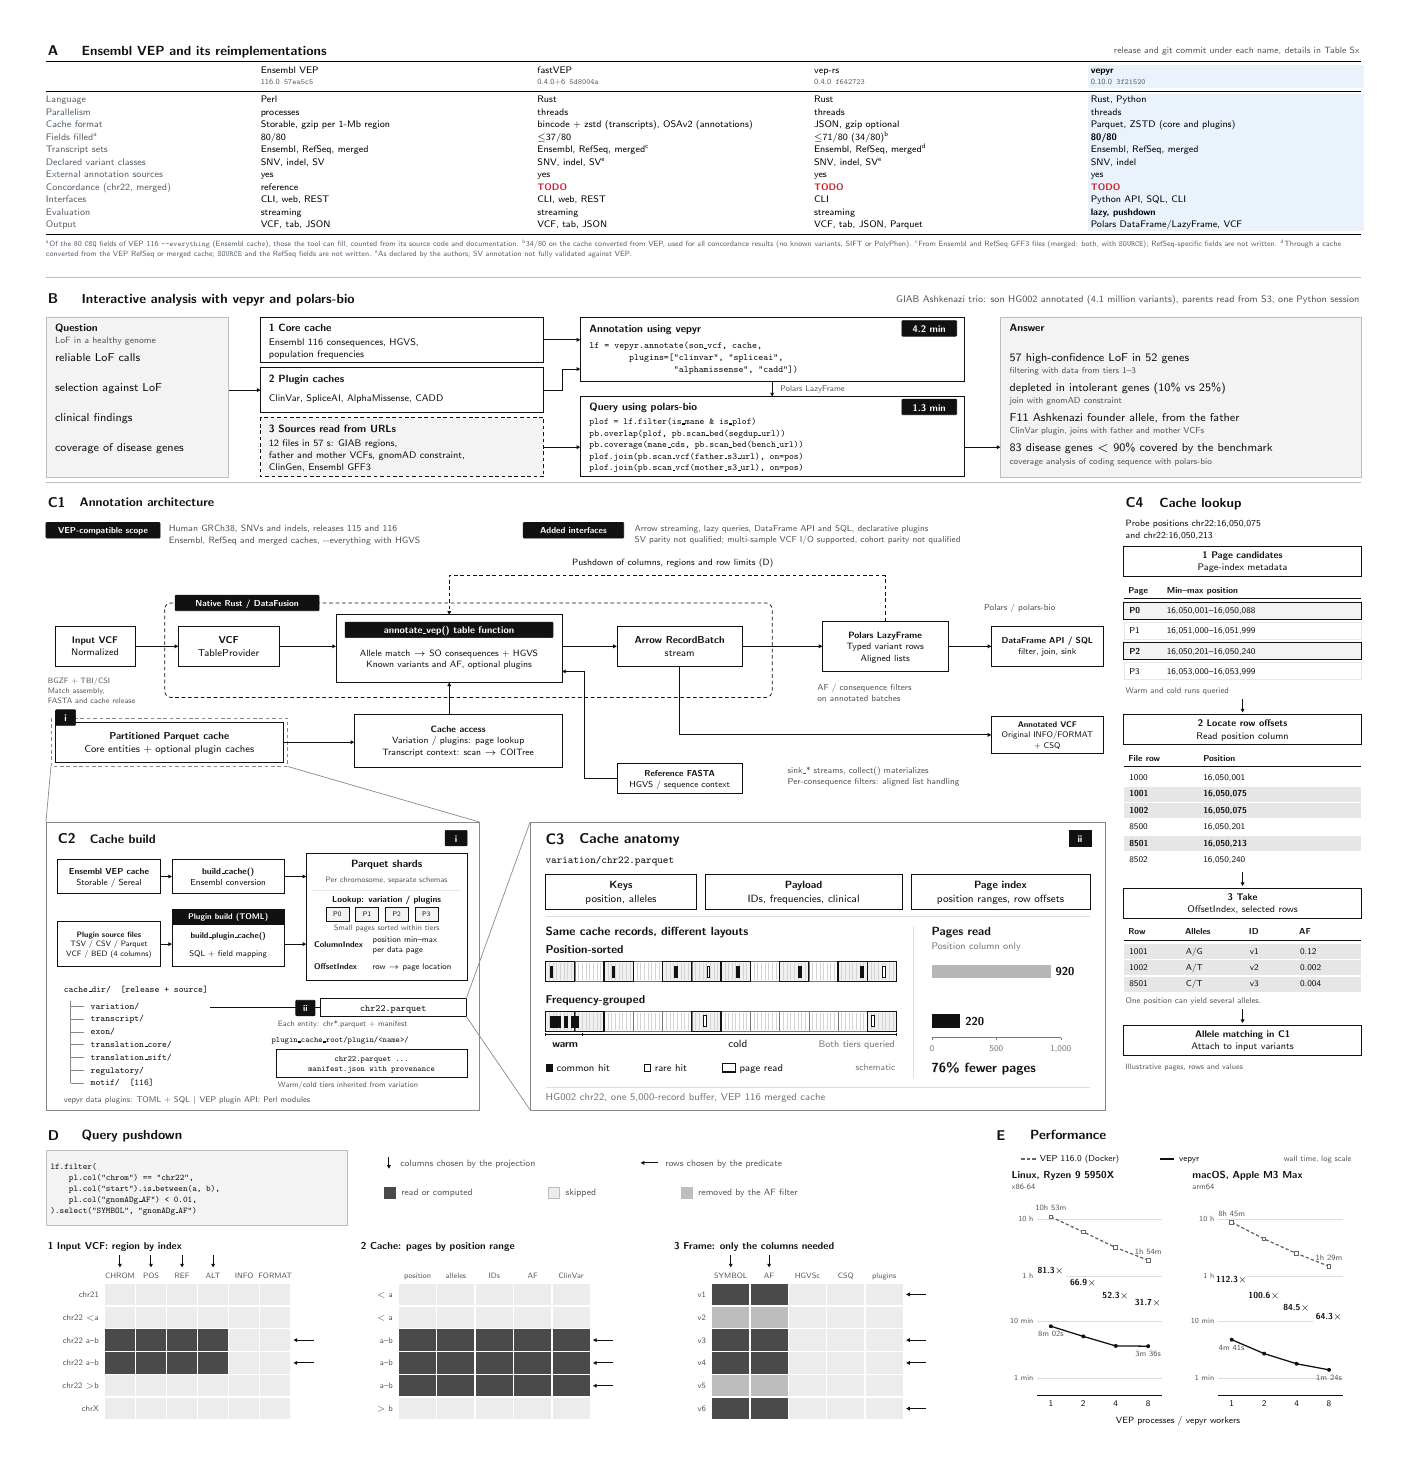
\begin{tikzpicture}[x=0.165034pt,y=-0.165034pt,every node/.style={inner sep=0pt,outer sep=0pt}]
\definecolor{f1c111111}{HTML}{111111}
\definecolor{f1c555555}{HTML}{555555}
\definecolor{f1cBDBDBD}{HTML}{BDBDBD}
\definecolor{f1cF3F3F3}{HTML}{F3F3F3}
\definecolor{f1c888888}{HTML}{888888}
\definecolor{f1cE6E6E6}{HTML}{E6E6E6}
\definecolor{f1cDEDEDE}{HTML}{DEDEDE}
\definecolor{f1c777777}{HTML}{777777}
\definecolor{f1cF0F0F0}{HTML}{F0F0F0}
\definecolor{f1cD4D4D4}{HTML}{D4D4D4}
\definecolor{f1cB6B6B6}{HTML}{B6B6B6}
\definecolor{f1c4A4A4A}{HTML}{4A4A4A}
\definecolor{f1cECECEC}{HTML}{ECECEC}
\definecolor{f1c666666}{HTML}{666666}
\definecolor{f1cDDDDDD}{HTML}{DDDDDD}
\useasboundingbox (0,0) rectangle (2960,3088);
\node[anchor=base west,text=f1c111111,font=\fontsize{5.12}{6.14}\selectfont\sffamily\bfseries] at (44,61.31) {A};
\node[anchor=base west,text=f1c111111,font=\fontsize{4.79}{5.74}\selectfont\sffamily\bfseries] at (118,60.59) {Ensembl VEP and its reimplementations};
\node[anchor=base east,text=f1c555555,font=\fontsize{3.3}{3.96}\selectfont\sffamily] at (2916,57.3) {release and git commit under each name, details in Table Sx};
\node[anchor=north west] at (40,74) {\resizebox{475.3pt}{!}{\figonetable}};
\draw[f1cBDBDBD,line width=0.17pt] (40,547.46) -- (2920,547.46);
\node[anchor=base west,text=f1c111111,font=\fontsize{5.12}{6.14}\selectfont\sffamily\bfseries] at (44,604.77) {B};
\node[anchor=base west,text=f1c111111,font=\fontsize{4.79}{5.74}\selectfont\sffamily\bfseries] at (118,604.04) {Interactive analysis with vepyr and polars-{}bio};
\node[anchor=base east,text=f1c555555,font=\fontsize{3.47}{4.16}\selectfont\sffamily] at (2916,601.12) {GIAB Ashkenazi trio: son HG002 annotated (4.1 million variants), parents read from S3, one Python session};
\path[fill=f1cF3F3F3,draw=f1cBDBDBD,line width=0.2pt] (40,633.46) rectangle (440,983.46);
\node[anchor=base west,text=f1c111111,font=\fontsize{3.8}{4.55}\selectfont\sffamily\bfseries] at (60,665.85) {Question};
\node[anchor=base west,text=f1c555555,font=\fontsize{3.3}{3.96}\selectfont\sffamily] at (60,691.76) {LoF in a healthy genome};
\node[anchor=base west,text=f1c111111,font=\fontsize{4.13}{4.95}\selectfont\sffamily] at (60,730.58) {reliable LoF calls};
\node[anchor=base west,text=f1c111111,font=\fontsize{4.13}{4.95}\selectfont\sffamily] at (60,796.58) {selection against LoF};
\node[anchor=base west,text=f1c111111,font=\fontsize{4.13}{4.95}\selectfont\sffamily] at (60,862.58) {clinical findings};
\node[anchor=base west,text=f1c111111,font=\fontsize{4.13}{4.95}\selectfont\sffamily] at (60,928.58) {coverage of disease genes};
\path[fill=white,draw=f1c111111,line width=0.3pt] (510,633.46) rectangle (1130,733.46);
\node[anchor=base west,text=f1c111111,font=\fontsize{3.8}{4.55}\selectfont\sffamily\bfseries] at (528,665.85) {1  Core cache};
\node[anchor=base west,text=f1c111111,font=\fontsize{3.47}{4.16}\selectfont\sffamily] at (528,694.79) {Ensembl 116 consequences, HGVS,};
\node[anchor=base west,text=f1c111111,font=\fontsize{3.47}{4.16}\selectfont\sffamily] at (528,721.46) {population frequencies};
\path[fill=white,draw=f1c111111,line width=0.3pt] (510,743.46) rectangle (1130,843.46);
\node[anchor=base west,text=f1c111111,font=\fontsize{3.8}{4.55}\selectfont\sffamily\bfseries] at (528,775.85) {2  Plugin caches};
\node[anchor=base west,text=f1c111111,font=\fontsize{3.47}{4.16}\selectfont\sffamily] at (528,818.12) {ClinVar, SpliceAI, AlphaMissense, CADD};
\path[fill=f1cF3F3F3,draw=f1c111111,line width=0.3pt,dash pattern=on 1.32pt off 0.99pt] (510,853.46) rectangle (1130,983.46);
\node[anchor=base west,text=f1c111111,font=\fontsize{3.8}{4.55}\selectfont\sffamily\bfseries] at (528,885.85) {3  Sources read from URLs};
\node[anchor=base west,text=f1c111111,font=\fontsize{3.47}{4.16}\selectfont\sffamily] at (528,916.45) {12 files in 57 s: GIAB regions,};
\node[anchor=base west,text=f1c111111,font=\fontsize{3.47}{4.16}\selectfont\sffamily] at (528,943.12) {father and mother VCFs, gnomAD constraint,};
\node[anchor=base west,text=f1c111111,font=\fontsize{3.47}{4.16}\selectfont\sffamily] at (528,969.79) {ClinGen, Ensembl GFF3};
\draw[f1c111111,line width=0.33pt,-{Triangle[length=1.32pt,width=1.32pt]}] (440,793.46) -- (510,793.46);
\path[fill=white,draw=f1c111111,line width=0.3pt] (1210,633.46) rectangle (2050,773.46);
\node[anchor=base west,text=f1c111111,font=\fontsize{3.8}{4.55}\selectfont\sffamily\bfseries] at (1230,667.85) {Annotation using vepyr};
\node[anchor=base west,text=f1c111111,font=\fontsize{3.38}{4.06}\selectfont\ttfamily] at (1230,702.91) {lf~=~vepyr.annotate(son\_vcf,~cache,};
\node[anchor=base west,text=f1c111111,font=\fontsize{3.38}{4.06}\selectfont\ttfamily] at (1230,728.94) {~~~~~~~~plugins=["clinvar",~"spliceai",};
\node[anchor=base west,text=f1c111111,font=\fontsize{3.38}{4.06}\selectfont\ttfamily] at (1230,754.98) {~~~~~~~~~~~~~~~~~"alphamissense",~"cadd"])};
\path[fill=white,draw=f1c111111,line width=0.3pt] (1210,807.46) rectangle (2050,983.46);
\node[anchor=base west,text=f1c111111,font=\fontsize{3.8}{4.55}\selectfont\sffamily\bfseries] at (1230,837.85) {Query using polars-{}bio};
\node[anchor=base west,text=f1c111111,font=\fontsize{3.3}{3.96}\selectfont\ttfamily] at (1230,868.96) {plof~=~lf.filter(is\_mane~\&~is\_plof)};
\node[anchor=base west,text=f1c111111,font=\fontsize{3.3}{3.96}\selectfont\ttfamily] at (1230,894.36) {pb.overlap(plof,~pb.scan\_bed(segdup\_url))};
\node[anchor=base west,text=f1c111111,font=\fontsize{3.3}{3.96}\selectfont\ttfamily] at (1230,919.76) {pb.coverage(mane\_cds,~pb.scan\_bed(bench\_url))};
\node[anchor=base west,text=f1c111111,font=\fontsize{3.3}{3.96}\selectfont\ttfamily] at (1230,945.16) {plof.join(pb.scan\_vcf(father\_s3\_url),~on=pos)};
\node[anchor=base west,text=f1c111111,font=\fontsize{3.3}{3.96}\selectfont\ttfamily] at (1230,970.56) {plof.join(pb.scan\_vcf(mother\_s3\_url),~on=pos)};
\path[fill=f1c111111,draw=f1c111111,line width=0.25pt,rounded corners=0.33pt] (1914,641.46) rectangle (2034,675.46);
\node[anchor=base,text=white,font=\fontsize{3.47}{4.16}\selectfont\sffamily\bfseries] at (1974,667.46) {4.2 min};
\path[fill=f1c111111,draw=f1c111111,line width=0.25pt,rounded corners=0.33pt] (1914,813.46) rectangle (2034,847.46);
\node[anchor=base,text=white,font=\fontsize{3.47}{4.16}\selectfont\sffamily\bfseries] at (1974,839.46) {1.3 min};
\draw[f1c111111,line width=0.33pt,-{Triangle[length=1.32pt,width=1.32pt]}] (1130,683.46) -- (1210,683.46);
\draw[f1c111111,line width=0.33pt] (1130,793.46) -- (1170,793.46) -- (1170,747.46);
\draw[f1c111111,line width=0.33pt,-{Triangle[length=1.32pt,width=1.32pt]}] (1170,747.46) -- (1210,747.46);
\draw[f1c111111,line width=0.33pt,-{Triangle[length=1.32pt,width=1.32pt]}] (1130,918.46) -- (1210,918.46);
\draw[f1c111111,line width=0.33pt,-{Triangle[length=1.32pt,width=1.32pt]}] (1630,773.46) -- (1630,807.46);
\node[anchor=base west,text=f1c555555,font=\fontsize{2.97}{3.56}\selectfont\sffamily] at (1648,797.03) {Polars LazyFrame};
\path[fill=f1cF3F3F3,draw=f1cBDBDBD,line width=0.2pt] (2130,633.46) rectangle (2920,983.46);
\draw[f1c111111,line width=0.33pt,-{Triangle[length=1.32pt,width=1.32pt]}] (2050,918.46) -- (2130,918.46);
\node[anchor=base west,text=f1c111111,font=\fontsize{3.8}{4.55}\selectfont\sffamily\bfseries] at (2150,665.85) {Answer};
\node[anchor=base west,text=f1c111111,font=\fontsize{4.13}{4.95}\selectfont\sffamily] at (2150,730.58) {57 high-{}confidence LoF in 52 genes};
\node[anchor=base west,text=f1c555555,font=\fontsize{3.14}{3.76}\selectfont\sffamily] at (2150,757.39) {filtering with data from tiers 1\textendash{}3};
\node[anchor=base west,text=f1c111111,font=\fontsize{4.13}{4.95}\selectfont\sffamily] at (2150,796.58) {depleted in intolerant genes (10\% vs 25\%)};
\node[anchor=base west,text=f1c555555,font=\fontsize{3.14}{3.76}\selectfont\sffamily] at (2150,823.39) {join with gnomAD constraint};
\node[anchor=base west,text=f1c111111,font=\fontsize{4.13}{4.95}\selectfont\sffamily] at (2150,862.58) {F11 Ashkenazi founder allele, from the father};
\node[anchor=base west,text=f1c555555,font=\fontsize{3.14}{3.76}\selectfont\sffamily] at (2150,889.39) {ClinVar plugin, joins with father and mother VCFs};
\node[anchor=base west,text=f1c111111,font=\fontsize{4.13}{4.95}\selectfont\sffamily] at (2150,928.58) {83 disease genes \ensuremath{<} 90\% covered by the benchmark};
\node[anchor=base west,text=f1c555555,font=\fontsize{3.14}{3.76}\selectfont\sffamily] at (2150,955.39) {coverage analysis of coding sequence with polars-{}bio};
\draw[f1cBDBDBD,line width=0.17pt] (40,995.46) -- (2920,995.46);
\node[anchor=base west,text=f1c111111,font=\fontsize{5.12}{6.14}\selectfont\sffamily\bfseries] at (44,1050.77) {C1};
\node[anchor=base west,text=f1c111111,font=\fontsize{4.46}{5.35}\selectfont\sffamily\bfseries] at (114,1049.31) {Annotation architecture};
\path[fill=f1c111111,draw=f1c111111,line width=0.25pt,rounded corners=0.33pt] (40,1083.46) rectangle (290,1117.46);
\node[anchor=base,text=white,font=\fontsize{3.14}{3.76}\selectfont\sffamily\bfseries] at (165,1107.46) {VEP-{}compatible scope};
\node[anchor=base west,text=f1c555555,font=\fontsize{3.3}{3.96}\selectfont\sffamily] at (309,1103.06) {Human GRCh38, SNVs and indels, releases 115 and 116};
\node[anchor=base west,text=f1c555555,font=\fontsize{3.3}{3.96}\selectfont\sffamily] at (309,1128.46) {Ensembl, RefSeq and merged caches, -{}-{}everything with HGVS};
\path[fill=f1c111111,draw=f1c111111,line width=0.25pt,rounded corners=0.33pt] (1085,1083.46) rectangle (1305,1117.46);
\node[anchor=base,text=white,font=\fontsize{3.14}{3.76}\selectfont\sffamily\bfseries] at (1195,1107.46) {Added interfaces};
\node[anchor=base west,text=f1c555555,font=\fontsize{3.14}{3.76}\selectfont\sffamily] at (1329,1103.33) {Arrow streaming, lazy queries, DataFrame API and SQL, declarative plugins};
\node[anchor=base west,text=f1c555555,font=\fontsize{3.14}{3.76}\selectfont\sffamily] at (1329,1127.46) {SV parity not qualified; multi-{}sample VCF I/O supported, cohort parity not qualified};
\path[fill=white,draw=f1c111111,line width=0.26pt,rounded corners=2.31pt,dash pattern=on 1.32pt off 0.99pt] (300,1259.46) rectangle (1630,1466.46);
\path[fill=f1c111111,draw=f1c111111,line width=0.25pt,rounded corners=0.33pt] (323,1242.46) rectangle (638,1276.46);
\node[anchor=base,text=white,font=\fontsize{3.14}{3.76}\selectfont\sffamily\bfseries] at (480.5,1266.46) {Native Rust / DataFusion};
\path[fill=white,draw=f1c111111,line width=0.25pt] (60,1310.46) rectangle (235,1398.46);
\node[anchor=base,text=f1c111111,font=\fontsize{3.47}{4.16}\selectfont\sffamily\bfseries] at (147.5,1348.79) {Input VCF};
\node[anchor=base,text=f1c111111,font=\fontsize{3.47}{4.16}\selectfont\sffamily] at (147.5,1375.46) {Normalized};
\path[fill=white,draw=f1c111111,line width=0.25pt] (330,1310.46) rectangle (550,1398.46);
\node[anchor=base,text=f1c111111,font=\fontsize{3.63}{4.36}\selectfont\sffamily\bfseries] at (440,1348.52) {VCF};
\node[anchor=base,text=f1c111111,font=\fontsize{3.63}{4.36}\selectfont\sffamily] at (440,1376.46) {TableProvider};
\path[fill=white,draw=f1c111111,line width=0.33pt] (675,1285.46) rectangle (1170,1433.46);
\path[fill=f1c111111,draw=f1c111111,line width=0.25pt,rounded corners=0.33pt] (695,1301.46) rectangle (1150,1335.46);
\node[anchor=base,text=white,font=\fontsize{3.47}{4.16}\selectfont\sffamily\bfseries] at (922.5,1327.46) {annotate\_vep() table function};
\node[anchor=base,text=f1c111111,font=\fontsize{3.3}{3.96}\selectfont\sffamily] at (922.5,1376.06) {Allele match \ensuremath{\rightarrow} SO consequences + HGVS};
\node[anchor=base,text=f1c111111,font=\fontsize{3.3}{3.96}\selectfont\sffamily] at (922.5,1401.46) {Known variants and AF, optional plugins};
\path[fill=white,draw=f1c111111,line width=0.25pt] (1290,1310.46) rectangle (1565,1398.46);
\node[anchor=base,text=f1c111111,font=\fontsize{3.63}{4.36}\selectfont\sffamily\bfseries] at (1427.5,1348.52) {Arrow RecordBatch};
\node[anchor=base,text=f1c111111,font=\fontsize{3.63}{4.36}\selectfont\sffamily] at (1427.5,1376.46) {stream};
\path[fill=white,draw=f1c111111,line width=0.25pt] (1740,1299.46) rectangle (2015,1409.46);
\node[anchor=base,text=f1c111111,font=\fontsize{3.3}{3.96}\selectfont\sffamily\bfseries] at (1877.5,1336.36) {Polars LazyFrame};
\node[anchor=base,text=f1c111111,font=\fontsize{3.3}{3.96}\selectfont\sffamily] at (1877.5,1361.76) {Typed variant rows};
\node[anchor=base,text=f1c111111,font=\fontsize{3.3}{3.96}\selectfont\sffamily] at (1877.5,1387.16) {Aligned lists};
\path[fill=white,draw=f1c111111,line width=0.25pt] (2110,1310.46) rectangle (2355,1398.46);
\node[anchor=base,text=f1c111111,font=\fontsize{3.14}{3.76}\selectfont\sffamily\bfseries] at (2232.5,1349.33) {DataFrame API / SQL};
\node[anchor=base,text=f1c111111,font=\fontsize{3.14}{3.76}\selectfont\sffamily] at (2232.5,1373.46) {filter, join, sink};
\node[anchor=base west,text=f1c555555,font=\fontsize{3.14}{3.76}\selectfont\sffamily] at (2094,1276.39) {Polars / polars-{}bio};
\draw[f1c111111,line width=0.36pt,-{Triangle[length=1.32pt,width=1.32pt]}] (235,1354.46) -- (330,1354.46);
\draw[f1c111111,line width=0.36pt,-{Triangle[length=1.32pt,width=1.32pt]}] (550,1354.46) -- (675,1354.46);
\draw[f1c111111,line width=0.36pt,-{Triangle[length=1.32pt,width=1.32pt]}] (1170,1354.46) -- (1290,1354.46);
\draw[f1c111111,line width=0.36pt,-{Triangle[length=1.32pt,width=1.32pt]}] (1565,1354.46) -- (1740,1354.46);
\draw[f1c111111,line width=0.36pt,-{Triangle[length=1.32pt,width=1.32pt]}] (2015,1354.46) -- (2110,1354.46);
\draw[f1c111111,line width=0.33pt,-{Triangle[length=1.32pt,width=1.32pt]},dash pattern=on 1.32pt off 0.99pt] (1877,1299.46) -- (1877,1199.46) -- (923,1199.46) -- (923,1285.46);
\node[anchor=base,text=f1c111111,font=\fontsize{3.3}{3.96}\selectfont\sffamily] at (1412.5,1177.76) {Pushdown of columns, regions and row limits (D)};
\node[anchor=base west,text=f1c555555,font=\fontsize{3.14}{3.76}\selectfont\sffamily] at (1729,1450.83) {AF / consequence filters};
\node[anchor=base west,text=f1c555555,font=\fontsize{3.14}{3.76}\selectfont\sffamily] at (1729,1474.96) {on annotated batches};
\path[fill=white,draw=f1c111111,line width=0.33pt] (60,1520.46) rectangle (560,1608.46);
\node[anchor=base,text=f1c111111,font=\fontsize{3.63}{4.36}\selectfont\sffamily\bfseries] at (310,1558.52) {Partitioned Parquet cache};
\node[anchor=base,text=f1c111111,font=\fontsize{3.63}{4.36}\selectfont\sffamily] at (310,1586.46) {Core entities + optional plugin caches};
\path[draw=f1c888888,line width=0.25pt,dash pattern=on 1.32pt off 0.99pt] (51,1511.46) rectangle (569,1617.46);
\path[fill=f1c111111,draw=f1c111111,line width=0.25pt,rounded corners=0.33pt] (61,1493.46) rectangle (105,1527.46);
\node[anchor=base,text=white,font=\fontsize{3.47}{4.16}\selectfont\sffamily\bfseries] at (83,1519.46) {i};
\path[fill=white,draw=f1c111111,line width=0.25pt] (715,1503.46) rectangle (1170,1618.46);
\node[anchor=base,text=f1c111111,font=\fontsize{3.3}{3.96}\selectfont\sffamily\bfseries] at (942.5,1542.86) {Cache access};
\node[anchor=base,text=f1c111111,font=\fontsize{3.3}{3.96}\selectfont\sffamily] at (942.5,1568.26) {Variation / plugins: page lookup};
\node[anchor=base,text=f1c111111,font=\fontsize{3.3}{3.96}\selectfont\sffamily] at (942.5,1593.66) {Transcript context: scan \ensuremath{\rightarrow} COITree};
\draw[f1c111111,line width=0.33pt,-{Triangle[length=1.32pt,width=1.32pt]}] (560,1564.46) -- (715,1564.46);
\draw[f1c111111,line width=0.33pt,-{Triangle[length=1.32pt,width=1.32pt]}] (923,1503.46) -- (923,1433.46);
\path[fill=white,draw=f1c111111,line width=0.25pt] (1290,1611.46) rectangle (1565,1676.46);
\node[anchor=base,text=f1c111111,font=\fontsize{3.14}{3.76}\selectfont\sffamily\bfseries] at (1427.5,1638.83) {Reference FASTA};
\node[anchor=base,text=f1c111111,font=\fontsize{3.14}{3.76}\selectfont\sffamily] at (1427.5,1662.96) {HGVS / sequence context};
\draw[f1c111111,line width=0.33pt,-{Triangle[length=1.32pt,width=1.32pt]}] (1290,1644.46) -- (1220,1644.46) -- (1220,1409.46) -- (1170,1409.46);
\path[fill=white,draw=f1c111111,line width=0.25pt] (2110,1508.46) rectangle (2355,1588.46);
\node[anchor=base,text=f1c111111,font=\fontsize{2.97}{3.56}\selectfont\sffamily\bfseries] at (2232.5,1532.17) {Annotated VCF};
\node[anchor=base,text=f1c111111,font=\fontsize{2.97}{3.56}\selectfont\sffamily] at (2232.5,1555.03) {Original INFO/FORMAT};
\node[anchor=base,text=f1c111111,font=\fontsize{2.97}{3.56}\selectfont\sffamily] at (2232.5,1577.89) {+ CSQ};
\draw[f1c111111,line width=0.33pt,-{Triangle[length=1.32pt,width=1.32pt]}] (1427,1398.46) -- (1427,1548.46) -- (2110,1548.46);
\node[anchor=base west,text=f1c555555,font=\fontsize{3.14}{3.76}\selectfont\sffamily] at (1664,1633.33) {sink\_* streams, collect() materializes};
\node[anchor=base west,text=f1c555555,font=\fontsize{3.14}{3.76}\selectfont\sffamily] at (1664,1657.46) {Per-{}consequence filters: aligned list handling};
\draw[f1c888888,line width=0.25pt] (51,1617.46) -- (40,1739.46);
\draw[f1c888888,line width=0.25pt] (569,1617.46) -- (990,1739.46);
\path[fill=white,draw=f1c888888,line width=0.25pt] (40,1739.46) rectangle (990,2369.46);
\node[anchor=base west,text=f1c111111,font=\fontsize{5.12}{6.14}\selectfont\sffamily\bfseries] at (66,1786.77) {C2};
\node[anchor=base west,text=f1c111111,font=\fontsize{4.46}{5.35}\selectfont\sffamily\bfseries] at (136,1785.31) {Cache build};
\path[fill=f1c111111,draw=f1c111111,line width=0.25pt,rounded corners=0.33pt] (914,1757.46) rectangle (962,1791.46);
\node[anchor=base,text=white,font=\fontsize{3.47}{4.16}\selectfont\sffamily\bfseries] at (938,1783.46) {i};
\path[fill=white,draw=f1c111111,line width=0.25pt] (66,1821.46) rectangle (290,1895.46);
\node[anchor=base,text=f1c111111,font=\fontsize{3.14}{3.76}\selectfont\sffamily\bfseries] at (178,1853.33) {Ensembl VEP cache};
\node[anchor=base,text=f1c111111,font=\fontsize{3.14}{3.76}\selectfont\sffamily] at (178,1877.46) {Storable / Sereal};
\path[fill=white,draw=f1c111111,line width=0.25pt] (316,1821.46) rectangle (562,1895.46);
\node[anchor=base,text=f1c111111,font=\fontsize{3.14}{3.76}\selectfont\sffamily\bfseries] at (439,1853.33) {build\_cache()};
\node[anchor=base,text=f1c111111,font=\fontsize{3.14}{3.76}\selectfont\sffamily] at (439,1877.46) {Ensembl conversion};
\path[fill=white,draw=f1c111111,line width=0.25pt] (66,1957.46) rectangle (290,2055.46);
\node[anchor=base,text=f1c111111,font=\fontsize{2.81}{3.37}\selectfont\sffamily\bfseries] at (178,1991.07) {Plugin source files};
\node[anchor=base,text=f1c111111,font=\fontsize{2.81}{3.37}\selectfont\sffamily] at (178,2012.66) {TSV / CSV / Parquet};
\node[anchor=base,text=f1c111111,font=\fontsize{2.81}{3.37}\selectfont\sffamily] at (178,2034.25) {VCF / BED (4 columns)};
\path[fill=white,draw=f1c111111,line width=0.25pt] (316,1929.46) rectangle (562,2055.46);
\path[fill=f1c111111,draw=f1c111111,line width=0.25pt] (316,1929.46) rectangle (562,1963.46);
\node[anchor=base,text=white,font=\fontsize{2.97}{3.56}\selectfont\sffamily\bfseries] at (439,1953.03) {Plugin build (TOML)};
\node[anchor=base,text=f1c111111,font=\fontsize{2.97}{3.56}\selectfont\sffamily\bfseries] at (439,1994.03) {build\_plugin\_cache()};
\node[anchor=base,text=f1c111111,font=\fontsize{2.97}{3.56}\selectfont\sffamily] at (439,2033.03) {SQL + field mapping};
\path[fill=white,draw=f1c111111,line width=0.33pt] (610,1807.46) rectangle (962,2085.46);
\node[anchor=base,text=f1c111111,font=\fontsize{3.8}{4.55}\selectfont\sffamily\bfseries] at (786,1838.35) {Parquet shards};
\node[anchor=base,text=f1c555555,font=\fontsize{2.81}{3.37}\selectfont\sffamily] at (786,1871.66) {Per chromosome, separate schemas};
\draw[f1cE6E6E6,line width=0.17pt] (623,1888.46) -- (949,1888.46);
\node[anchor=base,text=f1c111111,font=\fontsize{3.14}{3.76}\selectfont\sffamily\bfseries] at (786,1915.89) {Lookup: variation / plugins};
\path[fill=f1cF3F3F3,draw=f1c111111,line width=0.17pt] (653,1926.46) rectangle (703,1956.46);
\node[anchor=base,text=f1c111111,font=\fontsize{2.48}{2.97}\selectfont\sffamily] at (678,1946.93) {P0};
\path[fill=f1cF3F3F3,draw=f1c111111,line width=0.17pt] (718,1926.46) rectangle (768,1956.46);
\node[anchor=base,text=f1c111111,font=\fontsize{2.48}{2.97}\selectfont\sffamily] at (743,1946.93) {P1};
\path[fill=f1cF3F3F3,draw=f1c111111,line width=0.17pt] (783,1926.46) rectangle (833,1956.46);
\node[anchor=base,text=f1c111111,font=\fontsize{2.48}{2.97}\selectfont\sffamily] at (808,1946.93) {P2};
\path[fill=f1cF3F3F3,draw=f1c111111,line width=0.17pt] (848,1926.46) rectangle (898,1956.46);
\node[anchor=base,text=f1c111111,font=\fontsize{2.48}{2.97}\selectfont\sffamily] at (873,1946.93) {P3};
\node[anchor=base,text=f1c555555,font=\fontsize{2.81}{3.37}\selectfont\sffamily] at (786,1976.66) {Small pages sorted within tiers};
\node[anchor=base west,text=f1c111111,font=\fontsize{2.97}{3.56}\selectfont\sffamily\bfseries] at (627,2013.03) {ColumnIndex};
\node[anchor=base west,text=f1c111111,font=\fontsize{2.97}{3.56}\selectfont\sffamily] at (755,2002.46) {position min\textendash{}max};
\node[anchor=base west,text=f1c111111,font=\fontsize{2.97}{3.56}\selectfont\sffamily] at (755,2025.32) {per data page};
\node[anchor=base west,text=f1c111111,font=\fontsize{2.97}{3.56}\selectfont\sffamily\bfseries] at (627,2061.53) {OffsetIndex};
\node[anchor=base west,text=f1c111111,font=\fontsize{2.97}{3.56}\selectfont\sffamily] at (755,2061.53) {row \ensuremath{\rightarrow} page location};
\draw[f1c111111,line width=0.33pt,-{Triangle[length=1.32pt,width=1.32pt]}] (290,1858.46) -- (316,1858.46);
\draw[f1c111111,line width=0.33pt,-{Triangle[length=1.32pt,width=1.32pt]}] (290,2006.46) -- (316,2006.46);
\draw[f1c111111,line width=0.33pt,-{Triangle[length=1.32pt,width=1.32pt]}] (562,1858.46) -- (610,1858.46);
\draw[f1c111111,line width=0.33pt,-{Triangle[length=1.32pt,width=1.32pt]}] (562,2006.46) -- (610,2006.46);
\node[anchor=base west,text=f1c111111,font=\fontsize{3.3}{3.96}\selectfont\ttfamily\bfseries] at (79,2111.76) {cache\_dir/~~[release~+~source]};
\draw[f1c888888,line width=0.2pt] (94,2131.46) -- (94,2310.46);
\draw[f1c888888,line width=0.2pt] (94,2142.46) -- (124,2142.46);
\node[anchor=base west,text=f1c111111,font=\fontsize{3.3}{3.96}\selectfont\ttfamily\bfseries] at (138,2148.76) {variation/};
\draw[f1c888888,line width=0.2pt] (94,2170.46) -- (124,2170.46);
\node[anchor=base west,text=f1c111111,font=\fontsize{3.3}{3.96}\selectfont\ttfamily] at (138,2176.76) {transcript/};
\draw[f1c888888,line width=0.2pt] (94,2198.46) -- (124,2198.46);
\node[anchor=base west,text=f1c111111,font=\fontsize{3.3}{3.96}\selectfont\ttfamily] at (138,2204.76) {exon/};
\draw[f1c888888,line width=0.2pt] (94,2226.46) -- (124,2226.46);
\node[anchor=base west,text=f1c111111,font=\fontsize{3.3}{3.96}\selectfont\ttfamily] at (138,2232.76) {translation\_core/};
\draw[f1c888888,line width=0.2pt] (94,2254.46) -- (124,2254.46);
\node[anchor=base west,text=f1c111111,font=\fontsize{3.3}{3.96}\selectfont\ttfamily] at (138,2260.76) {translation\_sift/};
\draw[f1c888888,line width=0.2pt] (94,2282.46) -- (124,2282.46);
\node[anchor=base west,text=f1c111111,font=\fontsize{3.3}{3.96}\selectfont\ttfamily] at (138,2288.76) {regulatory/};
\draw[f1c888888,line width=0.2pt] (94,2310.46) -- (124,2310.46);
\node[anchor=base west,text=f1c111111,font=\fontsize{3.3}{3.96}\selectfont\ttfamily] at (138,2316.76) {motif/~~[116]};
\path[fill=white,draw=f1c111111,line width=0.33pt] (641,2126.46) rectangle (960,2164.46);
\node[anchor=base,text=f1c111111,font=\fontsize{3.47}{4.16}\selectfont\ttfamily\bfseries] at (800.5,2153.12) {chr22.parquet};
\draw[f1c111111,line width=0.2pt] (400,2145.46) -- (641,2145.46);
\path[fill=f1c111111,draw=f1c111111,line width=0.25pt,rounded corners=0.33pt] (587,2129.46) rectangle (629,2163.46);
\node[anchor=base,text=white,font=\fontsize{3.14}{3.76}\selectfont\sffamily\bfseries] at (608,2153.46) {ii};
\node[anchor=base west,text=f1c555555,font=\fontsize{2.81}{3.37}\selectfont\sffamily] at (548,2187.16) {Each entity: chr*.parquet + manifest};
\node[anchor=base west,text=f1c111111,font=\fontsize{2.97}{3.56}\selectfont\ttfamily\bfseries] at (534,2222.03) {plugin\_cache\_root/plugin/<name>/};
\path[fill=white,draw=f1c111111,line width=0.25pt] (544,2237.46) rectangle (962,2297.46);
\node[anchor=base,text=f1c111111,font=\fontsize{2.97}{3.56}\selectfont\ttfamily] at (753,2262.6) {chr22.parquet~\ldots{}};
\node[anchor=base,text=f1c111111,font=\fontsize{2.97}{3.56}\selectfont\ttfamily] at (753,2285.46) {manifest.json~with~provenance};
\node[anchor=base west,text=f1c555555,font=\fontsize{2.81}{3.37}\selectfont\sffamily] at (548,2319.66) {Warm/cold tiers inherited from variation};
\node[anchor=base west,text=f1c555555,font=\fontsize{2.97}{3.56}\selectfont\sffamily] at (79,2353.03) {vepyr data plugins: TOML + SQL  \ensuremath{|}  VEP plugin API: Perl modules};
\draw[f1c888888,line width=0.25pt] (960,2126.46) -- (1100,1739.46);
\draw[f1c888888,line width=0.25pt] (960,2164.46) -- (1100,2369.46);
\path[fill=white,draw=f1c888888,line width=0.25pt] (1100,1739.46) rectangle (2360,2369.46);
\node[anchor=base west,text=f1c555555,font=\fontsize{2.81}{3.37}\selectfont\sffamily] at (44,1436.07) {BGZF + TBI/CSI};
\node[anchor=base west,text=f1c555555,font=\fontsize{2.81}{3.37}\selectfont\sffamily] at (44,1457.66) {Match assembly,};
\node[anchor=base west,text=f1c555555,font=\fontsize{2.81}{3.37}\selectfont\sffamily] at (44,1479.25) {FASTA and cache release};
\node[anchor=base west,text=f1c111111,font=\fontsize{5.45}{6.54}\selectfont\sffamily\bfseries] at (1134,1787.5) {C3};
\node[anchor=base west,text=f1c111111,font=\fontsize{5.12}{6.14}\selectfont\sffamily\bfseries] at (1208,1786.77) {Cache anatomy};
\draw[f1cDEDEDE,line width=0.17pt] (1134,1946.46) -- (2326,1946.46);
\node[anchor=base west,text=f1c111111,font=\fontsize{4.29}{5.15}\selectfont\sffamily\bfseries] at (1134,1986.95) {Same cache records, different layouts};
\node[anchor=base west,text=f1c111111,font=\fontsize{4.29}{5.15}\selectfont\sffamily\bfseries] at (1979,1986.95) {Pages read};
\node[anchor=base west,text=f1c777777,font=\fontsize{3.47}{4.16}\selectfont\sffamily] at (1979,2017.62) {Position column only};
\draw[f1cDEDEDE,line width=0.17pt] (1939,1967.46) -- (1939,2300.46);
\node[anchor=base west,text=f1c111111,font=\fontsize{4.13}{4.95}\selectfont\sffamily\bfseries] at (1134,2028.08) {Position-{}sorted};
\path[fill=f1cF0F0F0,draw=f1c777777,line width=0.13pt] (1134,2044.46) rectangle (1198,2088.46);
\draw[f1cD4D4D4,line width=0.1pt] (1142,2047.46) -- (1142,2085.46);
\draw[f1cD4D4D4,line width=0.1pt] (1150,2047.46) -- (1150,2085.46);
\draw[f1cD4D4D4,line width=0.1pt] (1158,2047.46) -- (1158,2085.46);
\draw[f1cD4D4D4,line width=0.1pt] (1166,2047.46) -- (1166,2085.46);
\draw[f1cD4D4D4,line width=0.1pt] (1174,2047.46) -- (1174,2085.46);
\draw[f1cD4D4D4,line width=0.1pt] (1182,2047.46) -- (1182,2085.46);
\draw[f1cD4D4D4,line width=0.1pt] (1190,2047.46) -- (1190,2085.46);
\path[fill=white,draw=f1c777777,line width=0.13pt] (1198,2044.46) rectangle (1262,2088.46);
\draw[f1cD4D4D4,line width=0.1pt] (1206,2047.46) -- (1206,2085.46);
\draw[f1cD4D4D4,line width=0.1pt] (1214,2047.46) -- (1214,2085.46);
\draw[f1cD4D4D4,line width=0.1pt] (1222,2047.46) -- (1222,2085.46);
\draw[f1cD4D4D4,line width=0.1pt] (1230,2047.46) -- (1230,2085.46);
\draw[f1cD4D4D4,line width=0.1pt] (1238,2047.46) -- (1238,2085.46);
\draw[f1cD4D4D4,line width=0.1pt] (1246,2047.46) -- (1246,2085.46);
\draw[f1cD4D4D4,line width=0.1pt] (1254,2047.46) -- (1254,2085.46);
\path[fill=f1cF0F0F0,draw=f1c777777,line width=0.13pt] (1262,2044.46) rectangle (1326,2088.46);
\draw[f1cD4D4D4,line width=0.1pt] (1270,2047.46) -- (1270,2085.46);
\draw[f1cD4D4D4,line width=0.1pt] (1278,2047.46) -- (1278,2085.46);
\draw[f1cD4D4D4,line width=0.1pt] (1286,2047.46) -- (1286,2085.46);
\draw[f1cD4D4D4,line width=0.1pt] (1294,2047.46) -- (1294,2085.46);
\draw[f1cD4D4D4,line width=0.1pt] (1302,2047.46) -- (1302,2085.46);
\draw[f1cD4D4D4,line width=0.1pt] (1310,2047.46) -- (1310,2085.46);
\draw[f1cD4D4D4,line width=0.1pt] (1318,2047.46) -- (1318,2085.46);
\path[fill=white,draw=f1c777777,line width=0.13pt] (1326,2044.46) rectangle (1390,2088.46);
\draw[f1cD4D4D4,line width=0.1pt] (1334,2047.46) -- (1334,2085.46);
\draw[f1cD4D4D4,line width=0.1pt] (1342,2047.46) -- (1342,2085.46);
\draw[f1cD4D4D4,line width=0.1pt] (1350,2047.46) -- (1350,2085.46);
\draw[f1cD4D4D4,line width=0.1pt] (1358,2047.46) -- (1358,2085.46);
\draw[f1cD4D4D4,line width=0.1pt] (1366,2047.46) -- (1366,2085.46);
\draw[f1cD4D4D4,line width=0.1pt] (1374,2047.46) -- (1374,2085.46);
\draw[f1cD4D4D4,line width=0.1pt] (1382,2047.46) -- (1382,2085.46);
\path[fill=f1cF0F0F0,draw=f1c777777,line width=0.13pt] (1390,2044.46) rectangle (1454,2088.46);
\draw[f1cD4D4D4,line width=0.1pt] (1398,2047.46) -- (1398,2085.46);
\draw[f1cD4D4D4,line width=0.1pt] (1406,2047.46) -- (1406,2085.46);
\draw[f1cD4D4D4,line width=0.1pt] (1414,2047.46) -- (1414,2085.46);
\draw[f1cD4D4D4,line width=0.1pt] (1422,2047.46) -- (1422,2085.46);
\draw[f1cD4D4D4,line width=0.1pt] (1430,2047.46) -- (1430,2085.46);
\draw[f1cD4D4D4,line width=0.1pt] (1438,2047.46) -- (1438,2085.46);
\draw[f1cD4D4D4,line width=0.1pt] (1446,2047.46) -- (1446,2085.46);
\path[fill=f1cF0F0F0,draw=f1c777777,line width=0.13pt] (1454,2044.46) rectangle (1518,2088.46);
\draw[f1cD4D4D4,line width=0.1pt] (1462,2047.46) -- (1462,2085.46);
\draw[f1cD4D4D4,line width=0.1pt] (1470,2047.46) -- (1470,2085.46);
\draw[f1cD4D4D4,line width=0.1pt] (1478,2047.46) -- (1478,2085.46);
\draw[f1cD4D4D4,line width=0.1pt] (1486,2047.46) -- (1486,2085.46);
\draw[f1cD4D4D4,line width=0.1pt] (1494,2047.46) -- (1494,2085.46);
\draw[f1cD4D4D4,line width=0.1pt] (1502,2047.46) -- (1502,2085.46);
\draw[f1cD4D4D4,line width=0.1pt] (1510,2047.46) -- (1510,2085.46);
\path[fill=f1cF0F0F0,draw=f1c777777,line width=0.13pt] (1518,2044.46) rectangle (1582,2088.46);
\draw[f1cD4D4D4,line width=0.1pt] (1526,2047.46) -- (1526,2085.46);
\draw[f1cD4D4D4,line width=0.1pt] (1534,2047.46) -- (1534,2085.46);
\draw[f1cD4D4D4,line width=0.1pt] (1542,2047.46) -- (1542,2085.46);
\draw[f1cD4D4D4,line width=0.1pt] (1550,2047.46) -- (1550,2085.46);
\draw[f1cD4D4D4,line width=0.1pt] (1558,2047.46) -- (1558,2085.46);
\draw[f1cD4D4D4,line width=0.1pt] (1566,2047.46) -- (1566,2085.46);
\draw[f1cD4D4D4,line width=0.1pt] (1574,2047.46) -- (1574,2085.46);
\path[fill=white,draw=f1c777777,line width=0.13pt] (1582,2044.46) rectangle (1646,2088.46);
\draw[f1cD4D4D4,line width=0.1pt] (1590,2047.46) -- (1590,2085.46);
\draw[f1cD4D4D4,line width=0.1pt] (1598,2047.46) -- (1598,2085.46);
\draw[f1cD4D4D4,line width=0.1pt] (1606,2047.46) -- (1606,2085.46);
\draw[f1cD4D4D4,line width=0.1pt] (1614,2047.46) -- (1614,2085.46);
\draw[f1cD4D4D4,line width=0.1pt] (1622,2047.46) -- (1622,2085.46);
\draw[f1cD4D4D4,line width=0.1pt] (1630,2047.46) -- (1630,2085.46);
\draw[f1cD4D4D4,line width=0.1pt] (1638,2047.46) -- (1638,2085.46);
\path[fill=f1cF0F0F0,draw=f1c777777,line width=0.13pt] (1646,2044.46) rectangle (1710,2088.46);
\draw[f1cD4D4D4,line width=0.1pt] (1654,2047.46) -- (1654,2085.46);
\draw[f1cD4D4D4,line width=0.1pt] (1662,2047.46) -- (1662,2085.46);
\draw[f1cD4D4D4,line width=0.1pt] (1670,2047.46) -- (1670,2085.46);
\draw[f1cD4D4D4,line width=0.1pt] (1678,2047.46) -- (1678,2085.46);
\draw[f1cD4D4D4,line width=0.1pt] (1686,2047.46) -- (1686,2085.46);
\draw[f1cD4D4D4,line width=0.1pt] (1694,2047.46) -- (1694,2085.46);
\draw[f1cD4D4D4,line width=0.1pt] (1702,2047.46) -- (1702,2085.46);
\path[fill=white,draw=f1c777777,line width=0.13pt] (1710,2044.46) rectangle (1774,2088.46);
\draw[f1cD4D4D4,line width=0.1pt] (1718,2047.46) -- (1718,2085.46);
\draw[f1cD4D4D4,line width=0.1pt] (1726,2047.46) -- (1726,2085.46);
\draw[f1cD4D4D4,line width=0.1pt] (1734,2047.46) -- (1734,2085.46);
\draw[f1cD4D4D4,line width=0.1pt] (1742,2047.46) -- (1742,2085.46);
\draw[f1cD4D4D4,line width=0.1pt] (1750,2047.46) -- (1750,2085.46);
\draw[f1cD4D4D4,line width=0.1pt] (1758,2047.46) -- (1758,2085.46);
\draw[f1cD4D4D4,line width=0.1pt] (1766,2047.46) -- (1766,2085.46);
\path[fill=f1cF0F0F0,draw=f1c777777,line width=0.13pt] (1774,2044.46) rectangle (1838,2088.46);
\draw[f1cD4D4D4,line width=0.1pt] (1782,2047.46) -- (1782,2085.46);
\draw[f1cD4D4D4,line width=0.1pt] (1790,2047.46) -- (1790,2085.46);
\draw[f1cD4D4D4,line width=0.1pt] (1798,2047.46) -- (1798,2085.46);
\draw[f1cD4D4D4,line width=0.1pt] (1806,2047.46) -- (1806,2085.46);
\draw[f1cD4D4D4,line width=0.1pt] (1814,2047.46) -- (1814,2085.46);
\draw[f1cD4D4D4,line width=0.1pt] (1822,2047.46) -- (1822,2085.46);
\draw[f1cD4D4D4,line width=0.1pt] (1830,2047.46) -- (1830,2085.46);
\path[fill=f1cF0F0F0,draw=f1c777777,line width=0.13pt] (1838,2044.46) rectangle (1902,2088.46);
\draw[f1cD4D4D4,line width=0.1pt] (1846,2047.46) -- (1846,2085.46);
\draw[f1cD4D4D4,line width=0.1pt] (1854,2047.46) -- (1854,2085.46);
\draw[f1cD4D4D4,line width=0.1pt] (1862,2047.46) -- (1862,2085.46);
\draw[f1cD4D4D4,line width=0.1pt] (1870,2047.46) -- (1870,2085.46);
\draw[f1cD4D4D4,line width=0.1pt] (1878,2047.46) -- (1878,2085.46);
\draw[f1cD4D4D4,line width=0.1pt] (1886,2047.46) -- (1886,2085.46);
\draw[f1cD4D4D4,line width=0.1pt] (1894,2047.46) -- (1894,2085.46);
\path[fill=f1c111111,draw=f1c111111,line width=0.12pt] (1143,2054.46) rectangle (1149,2078.46);
\path[fill=f1c111111,draw=f1c111111,line width=0.12pt] (1279,2054.46) rectangle (1285,2078.46);
\path[fill=f1c111111,draw=f1c111111,line width=0.12pt] (1415,2054.46) rectangle (1421,2078.46);
\path[fill=f1c111111,draw=f1c111111,line width=0.12pt] (1551,2054.46) rectangle (1557,2078.46);
\path[fill=f1c111111,draw=f1c111111,line width=0.12pt] (1687,2054.46) rectangle (1693,2078.46);
\path[fill=f1c111111,draw=f1c111111,line width=0.12pt] (1823,2054.46) rectangle (1829,2078.46);
\path[fill=white,draw=f1c111111,line width=0.23pt] (1487,2054.46) rectangle (1493,2078.46);
\path[fill=white,draw=f1c111111,line width=0.23pt] (1871,2054.46) rectangle (1877,2078.46);
\path[draw=f1c111111,line width=0.43pt] (1134,2044.46) rectangle (1198,2088.46);
\path[draw=f1c111111,line width=0.43pt] (1262,2044.46) rectangle (1326,2088.46);
\path[draw=f1c111111,line width=0.43pt] (1390,2044.46) rectangle (1454,2088.46);
\path[draw=f1c111111,line width=0.43pt] (1454,2044.46) rectangle (1518,2088.46);
\path[draw=f1c111111,line width=0.43pt] (1518,2044.46) rectangle (1582,2088.46);
\path[draw=f1c111111,line width=0.43pt] (1646,2044.46) rectangle (1710,2088.46);
\path[draw=f1c111111,line width=0.43pt] (1774,2044.46) rectangle (1838,2088.46);
\path[draw=f1c111111,line width=0.43pt] (1838,2044.46) rectangle (1902,2088.46);
\node[anchor=base west,text=f1c111111,font=\fontsize{4.13}{4.95}\selectfont\sffamily\bfseries] at (1134,2137.08) {Frequency-{}grouped};
\path[fill=f1cF0F0F0,draw=f1c777777,line width=0.13pt] (1134,2153.46) rectangle (1198,2197.46);
\draw[f1cD4D4D4,line width=0.1pt] (1142,2156.46) -- (1142,2194.46);
\draw[f1cD4D4D4,line width=0.1pt] (1150,2156.46) -- (1150,2194.46);
\draw[f1cD4D4D4,line width=0.1pt] (1158,2156.46) -- (1158,2194.46);
\draw[f1cD4D4D4,line width=0.1pt] (1166,2156.46) -- (1166,2194.46);
\draw[f1cD4D4D4,line width=0.1pt] (1174,2156.46) -- (1174,2194.46);
\draw[f1cD4D4D4,line width=0.1pt] (1182,2156.46) -- (1182,2194.46);
\draw[f1cD4D4D4,line width=0.1pt] (1190,2156.46) -- (1190,2194.46);
\path[fill=f1cF0F0F0,draw=f1c777777,line width=0.13pt] (1198,2153.46) rectangle (1262,2197.46);
\draw[f1cD4D4D4,line width=0.1pt] (1206,2156.46) -- (1206,2194.46);
\draw[f1cD4D4D4,line width=0.1pt] (1214,2156.46) -- (1214,2194.46);
\draw[f1cD4D4D4,line width=0.1pt] (1222,2156.46) -- (1222,2194.46);
\draw[f1cD4D4D4,line width=0.1pt] (1230,2156.46) -- (1230,2194.46);
\draw[f1cD4D4D4,line width=0.1pt] (1238,2156.46) -- (1238,2194.46);
\draw[f1cD4D4D4,line width=0.1pt] (1246,2156.46) -- (1246,2194.46);
\draw[f1cD4D4D4,line width=0.1pt] (1254,2156.46) -- (1254,2194.46);
\path[fill=white,draw=f1c777777,line width=0.13pt] (1262,2153.46) rectangle (1326,2197.46);
\draw[f1cD4D4D4,line width=0.1pt] (1270,2156.46) -- (1270,2194.46);
\draw[f1cD4D4D4,line width=0.1pt] (1278,2156.46) -- (1278,2194.46);
\draw[f1cD4D4D4,line width=0.1pt] (1286,2156.46) -- (1286,2194.46);
\draw[f1cD4D4D4,line width=0.1pt] (1294,2156.46) -- (1294,2194.46);
\draw[f1cD4D4D4,line width=0.1pt] (1302,2156.46) -- (1302,2194.46);
\draw[f1cD4D4D4,line width=0.1pt] (1310,2156.46) -- (1310,2194.46);
\draw[f1cD4D4D4,line width=0.1pt] (1318,2156.46) -- (1318,2194.46);
\path[fill=white,draw=f1c777777,line width=0.13pt] (1326,2153.46) rectangle (1390,2197.46);
\draw[f1cD4D4D4,line width=0.1pt] (1334,2156.46) -- (1334,2194.46);
\draw[f1cD4D4D4,line width=0.1pt] (1342,2156.46) -- (1342,2194.46);
\draw[f1cD4D4D4,line width=0.1pt] (1350,2156.46) -- (1350,2194.46);
\draw[f1cD4D4D4,line width=0.1pt] (1358,2156.46) -- (1358,2194.46);
\draw[f1cD4D4D4,line width=0.1pt] (1366,2156.46) -- (1366,2194.46);
\draw[f1cD4D4D4,line width=0.1pt] (1374,2156.46) -- (1374,2194.46);
\draw[f1cD4D4D4,line width=0.1pt] (1382,2156.46) -- (1382,2194.46);
\path[fill=white,draw=f1c777777,line width=0.13pt] (1390,2153.46) rectangle (1454,2197.46);
\draw[f1cD4D4D4,line width=0.1pt] (1398,2156.46) -- (1398,2194.46);
\draw[f1cD4D4D4,line width=0.1pt] (1406,2156.46) -- (1406,2194.46);
\draw[f1cD4D4D4,line width=0.1pt] (1414,2156.46) -- (1414,2194.46);
\draw[f1cD4D4D4,line width=0.1pt] (1422,2156.46) -- (1422,2194.46);
\draw[f1cD4D4D4,line width=0.1pt] (1430,2156.46) -- (1430,2194.46);
\draw[f1cD4D4D4,line width=0.1pt] (1438,2156.46) -- (1438,2194.46);
\draw[f1cD4D4D4,line width=0.1pt] (1446,2156.46) -- (1446,2194.46);
\path[fill=f1cF0F0F0,draw=f1c777777,line width=0.13pt] (1454,2153.46) rectangle (1518,2197.46);
\draw[f1cD4D4D4,line width=0.1pt] (1462,2156.46) -- (1462,2194.46);
\draw[f1cD4D4D4,line width=0.1pt] (1470,2156.46) -- (1470,2194.46);
\draw[f1cD4D4D4,line width=0.1pt] (1478,2156.46) -- (1478,2194.46);
\draw[f1cD4D4D4,line width=0.1pt] (1486,2156.46) -- (1486,2194.46);
\draw[f1cD4D4D4,line width=0.1pt] (1494,2156.46) -- (1494,2194.46);
\draw[f1cD4D4D4,line width=0.1pt] (1502,2156.46) -- (1502,2194.46);
\draw[f1cD4D4D4,line width=0.1pt] (1510,2156.46) -- (1510,2194.46);
\path[fill=white,draw=f1c777777,line width=0.13pt] (1518,2153.46) rectangle (1582,2197.46);
\draw[f1cD4D4D4,line width=0.1pt] (1526,2156.46) -- (1526,2194.46);
\draw[f1cD4D4D4,line width=0.1pt] (1534,2156.46) -- (1534,2194.46);
\draw[f1cD4D4D4,line width=0.1pt] (1542,2156.46) -- (1542,2194.46);
\draw[f1cD4D4D4,line width=0.1pt] (1550,2156.46) -- (1550,2194.46);
\draw[f1cD4D4D4,line width=0.1pt] (1558,2156.46) -- (1558,2194.46);
\draw[f1cD4D4D4,line width=0.1pt] (1566,2156.46) -- (1566,2194.46);
\draw[f1cD4D4D4,line width=0.1pt] (1574,2156.46) -- (1574,2194.46);
\path[fill=white,draw=f1c777777,line width=0.13pt] (1582,2153.46) rectangle (1646,2197.46);
\draw[f1cD4D4D4,line width=0.1pt] (1590,2156.46) -- (1590,2194.46);
\draw[f1cD4D4D4,line width=0.1pt] (1598,2156.46) -- (1598,2194.46);
\draw[f1cD4D4D4,line width=0.1pt] (1606,2156.46) -- (1606,2194.46);
\draw[f1cD4D4D4,line width=0.1pt] (1614,2156.46) -- (1614,2194.46);
\draw[f1cD4D4D4,line width=0.1pt] (1622,2156.46) -- (1622,2194.46);
\draw[f1cD4D4D4,line width=0.1pt] (1630,2156.46) -- (1630,2194.46);
\draw[f1cD4D4D4,line width=0.1pt] (1638,2156.46) -- (1638,2194.46);
\path[fill=white,draw=f1c777777,line width=0.13pt] (1646,2153.46) rectangle (1710,2197.46);
\draw[f1cD4D4D4,line width=0.1pt] (1654,2156.46) -- (1654,2194.46);
\draw[f1cD4D4D4,line width=0.1pt] (1662,2156.46) -- (1662,2194.46);
\draw[f1cD4D4D4,line width=0.1pt] (1670,2156.46) -- (1670,2194.46);
\draw[f1cD4D4D4,line width=0.1pt] (1678,2156.46) -- (1678,2194.46);
\draw[f1cD4D4D4,line width=0.1pt] (1686,2156.46) -- (1686,2194.46);
\draw[f1cD4D4D4,line width=0.1pt] (1694,2156.46) -- (1694,2194.46);
\draw[f1cD4D4D4,line width=0.1pt] (1702,2156.46) -- (1702,2194.46);
\path[fill=white,draw=f1c777777,line width=0.13pt] (1710,2153.46) rectangle (1774,2197.46);
\draw[f1cD4D4D4,line width=0.1pt] (1718,2156.46) -- (1718,2194.46);
\draw[f1cD4D4D4,line width=0.1pt] (1726,2156.46) -- (1726,2194.46);
\draw[f1cD4D4D4,line width=0.1pt] (1734,2156.46) -- (1734,2194.46);
\draw[f1cD4D4D4,line width=0.1pt] (1742,2156.46) -- (1742,2194.46);
\draw[f1cD4D4D4,line width=0.1pt] (1750,2156.46) -- (1750,2194.46);
\draw[f1cD4D4D4,line width=0.1pt] (1758,2156.46) -- (1758,2194.46);
\draw[f1cD4D4D4,line width=0.1pt] (1766,2156.46) -- (1766,2194.46);
\path[fill=white,draw=f1c777777,line width=0.13pt] (1774,2153.46) rectangle (1838,2197.46);
\draw[f1cD4D4D4,line width=0.1pt] (1782,2156.46) -- (1782,2194.46);
\draw[f1cD4D4D4,line width=0.1pt] (1790,2156.46) -- (1790,2194.46);
\draw[f1cD4D4D4,line width=0.1pt] (1798,2156.46) -- (1798,2194.46);
\draw[f1cD4D4D4,line width=0.1pt] (1806,2156.46) -- (1806,2194.46);
\draw[f1cD4D4D4,line width=0.1pt] (1814,2156.46) -- (1814,2194.46);
\draw[f1cD4D4D4,line width=0.1pt] (1822,2156.46) -- (1822,2194.46);
\draw[f1cD4D4D4,line width=0.1pt] (1830,2156.46) -- (1830,2194.46);
\path[fill=f1cF0F0F0,draw=f1c777777,line width=0.13pt] (1838,2153.46) rectangle (1902,2197.46);
\draw[f1cD4D4D4,line width=0.1pt] (1846,2156.46) -- (1846,2194.46);
\draw[f1cD4D4D4,line width=0.1pt] (1854,2156.46) -- (1854,2194.46);
\draw[f1cD4D4D4,line width=0.1pt] (1862,2156.46) -- (1862,2194.46);
\draw[f1cD4D4D4,line width=0.1pt] (1870,2156.46) -- (1870,2194.46);
\draw[f1cD4D4D4,line width=0.1pt] (1878,2156.46) -- (1878,2194.46);
\draw[f1cD4D4D4,line width=0.1pt] (1886,2156.46) -- (1886,2194.46);
\draw[f1cD4D4D4,line width=0.1pt] (1894,2156.46) -- (1894,2194.46);
\path[fill=f1c111111,draw=f1c111111,line width=0.12pt] (1143,2163.46) rectangle (1149,2187.46);
\path[fill=f1c111111,draw=f1c111111,line width=0.12pt] (1151,2163.46) rectangle (1157,2187.46);
\path[fill=f1c111111,draw=f1c111111,line width=0.12pt] (1159,2163.46) rectangle (1165,2187.46);
\path[fill=f1c111111,draw=f1c111111,line width=0.12pt] (1175,2163.46) rectangle (1181,2187.46);
\path[fill=f1c111111,draw=f1c111111,line width=0.12pt] (1191,2163.46) rectangle (1197,2187.46);
\path[fill=f1c111111,draw=f1c111111,line width=0.12pt] (1199,2163.46) rectangle (1205,2187.46);
\path[fill=white,draw=f1c111111,line width=0.23pt] (1479,2163.46) rectangle (1485,2187.46);
\path[fill=white,draw=f1c111111,line width=0.23pt] (1847,2163.46) rectangle (1853,2187.46);
\path[draw=f1c111111,line width=0.43pt] (1134,2153.46) rectangle (1198,2197.46);
\path[draw=f1c111111,line width=0.43pt] (1198,2153.46) rectangle (1262,2197.46);
\path[draw=f1c111111,line width=0.43pt] (1454,2153.46) rectangle (1518,2197.46);
\path[draw=f1c111111,line width=0.43pt] (1838,2153.46) rectangle (1902,2197.46);
\draw[f1c111111,line width=0.2pt] (1134,2204.46) -- (1214,2204.46);
\draw[f1c111111,line width=0.2pt] (1134,2200.46) -- (1134,2208.46);
\draw[f1c111111,line width=0.2pt] (1214,2200.46) -- (1214,2208.46);
\draw[f1c111111,line width=0.2pt] (1214,2204.46) -- (1902,2204.46);
\draw[f1c111111,line width=0.2pt] (1214,2200.46) -- (1214,2208.46);
\draw[f1c111111,line width=0.2pt] (1902,2200.46) -- (1902,2208.46);
\node[anchor=base,text=f1c111111,font=\fontsize{3.8}{4.55}\selectfont\sffamily\bfseries] at (1177,2232.85) {warm};
\node[anchor=base,text=f1c111111,font=\fontsize{3.8}{4.55}\selectfont\sffamily] at (1555,2232.85) {cold};
\node[anchor=base east,text=f1c777777,font=\fontsize{3.47}{4.16}\selectfont\sffamily] at (1899,2232.12) {Both tiers queried};
\path[fill=f1c111111,draw=f1c111111,line width=0.2pt] (1136,2269.46) rectangle (1148,2285.46);
\node[anchor=base west,text=f1c111111,font=\fontsize{3.63}{4.36}\selectfont\sffamily] at (1158,2284.99) {common hit};
\path[fill=white,draw=f1c111111,line width=0.26pt] (1351,2269.46) rectangle (1363,2285.46);
\node[anchor=base west,text=f1c111111,font=\fontsize{3.63}{4.36}\selectfont\sffamily] at (1373,2284.99) {rare hit};
\path[draw=f1c111111,line width=0.43pt] (1521,2268.46) rectangle (1549,2286.46);
\node[anchor=base west,text=f1c111111,font=\fontsize{3.63}{4.36}\selectfont\sffamily] at (1559,2284.99) {page read};
\node[anchor=base east,text=f1c777777,font=\fontsize{3.3}{3.96}\selectfont\sffamily] at (1900,2284.26) {schematic};
\path[fill=f1cB6B6B6] (1980,2051.46) rectangle (2239.44,2081.46);
\node[anchor=base west,text=f1c111111,font=\fontsize{4.13}{4.95}\selectfont\sffamily\bfseries] at (2250.44,2075.08) {920};
\path[fill=f1c111111] (1980,2160.46) rectangle (2042.04,2190.46);
\node[anchor=base west,text=f1c111111,font=\fontsize{4.13}{4.95}\selectfont\sffamily\bfseries] at (2053.04,2184.08) {220};
\draw[f1c777777,line width=0.17pt] (1980,2211.46) -- (2262,2211.46);
\draw[f1c777777,line width=0.17pt] (1980,2211.46) -- (1980,2217.46);
\node[anchor=base,text=f1c777777,font=\fontsize{3.14}{3.76}\selectfont\sffamily] at (1980,2241.39) {0};
\draw[f1c777777,line width=0.17pt] (2121,2211.46) -- (2121,2217.46);
\node[anchor=base,text=f1c777777,font=\fontsize{3.14}{3.76}\selectfont\sffamily] at (2121,2241.39) {500};
\draw[f1c777777,line width=0.17pt] (2262,2211.46) -- (2262,2217.46);
\node[anchor=base,text=f1c777777,font=\fontsize{3.14}{3.76}\selectfont\sffamily] at (2262,2241.39) {1,000};
\node[anchor=base west,text=f1c111111,font=\fontsize{4.79}{5.74}\selectfont\sffamily\bfseries] at (1979,2287.54) {76\% fewer pages};
\draw[f1cDEDEDE,line width=0.17pt] (1134,2319.46) -- (2326,2319.46);
\node[anchor=base west,text=f1c777777,font=\fontsize{3.63}{4.36}\selectfont\sffamily] at (1134,2349.49) {HG002 chr22, one 5,000-{}record buffer, VEP 116 merged cache};
\node[anchor=base west,text=f1c111111,font=\fontsize{3.8}{4.55}\selectfont\ttfamily] at (1134,1829.85) {variation/chr22.parquet};
\path[fill=f1c111111,draw=f1c111111,line width=0.25pt] (2280,1758.46) rectangle (2328,1792.46);
\node[anchor=base,text=white,font=\fontsize{3.47}{4.16}\selectfont\sffamily\bfseries] at (2304,1784.46) {ii};
\path[fill=white,draw=f1c111111,line width=0.25pt] (1134,1853.46) rectangle (1464,1929.46);
\node[anchor=base,text=f1c111111,font=\fontsize{3.8}{4.55}\selectfont\sffamily\bfseries] at (1299,1885.25) {Keys};
\node[anchor=base,text=f1c111111,font=\fontsize{3.8}{4.55}\selectfont\sffamily] at (1299,1914.46) {position, alleles};
\path[fill=white,draw=f1c111111,line width=0.25pt] (1484,1853.46) rectangle (1914,1929.46);
\node[anchor=base,text=f1c111111,font=\fontsize{3.8}{4.55}\selectfont\sffamily\bfseries] at (1699,1885.25) {Payload};
\node[anchor=base,text=f1c111111,font=\fontsize{3.8}{4.55}\selectfont\sffamily] at (1699,1914.46) {IDs, frequencies, clinical};
\path[fill=white,draw=f1c111111,line width=0.25pt] (1934,1853.46) rectangle (2326,1929.46);
\node[anchor=base,text=f1c111111,font=\fontsize{3.8}{4.55}\selectfont\sffamily\bfseries] at (2130,1885.25) {Page index};
\node[anchor=base,text=f1c111111,font=\fontsize{3.8}{4.55}\selectfont\sffamily] at (2130,1914.46) {position ranges, row offsets};
\node[anchor=base west,text=f1c111111,font=\fontsize{5.12}{6.14}\selectfont\sffamily\bfseries] at (2404,1050.77) {C4};
\node[anchor=base west,text=f1c111111,font=\fontsize{4.79}{5.74}\selectfont\sffamily\bfseries] at (2478,1050.04) {Cache lookup};
\node[anchor=base west,text=f1c111111,font=\fontsize{3.3}{3.96}\selectfont\sffamily] at (2404,1092.06) {Probe positions chr22:16,050,075};
\node[anchor=base west,text=f1c111111,font=\fontsize{3.3}{3.96}\selectfont\sffamily] at (2404,1117.46) {and chr22:16,050,213};
\path[fill=white,draw=f1c111111,line width=0.3pt] (2400,1135.46) rectangle (2920,1201.46);
\node[anchor=base,text=f1c111111,font=\fontsize{3.47}{4.16}\selectfont\sffamily\bfseries] at (2660,1162.79) {1  Page candidates};
\node[anchor=base,text=f1c111111,font=\fontsize{3.47}{4.16}\selectfont\sffamily] at (2660,1189.46) {Page-{}index metadata};
\node[anchor=base west,text=f1c111111,font=\fontsize{3.14}{3.76}\selectfont\sffamily\bfseries] at (2410,1238.39) {Page};
\node[anchor=base west,text=f1c111111,font=\fontsize{3.14}{3.76}\selectfont\sffamily\bfseries] at (2494,1238.39) {Min\textendash{}max position};
\draw[f1c111111,line width=0.25pt] (2400,1249.46) -- (2920,1249.46);
\path[fill=f1cF3F3F3,draw=f1c111111,line width=0.33pt] (2400,1257.46) rectangle (2920,1295.46);
\node[anchor=base west,text=f1c111111,font=\fontsize{3.14}{3.76}\selectfont\sffamily\bfseries] at (2412,1283.39) {P0};
\node[anchor=base west,text=f1c111111,font=\fontsize{3.14}{3.76}\selectfont\sffamily] at (2494,1283.39) {16,050,001\textendash{}16,050,088};
\path[fill=white,draw=f1cE6E6E6,line width=0.13pt] (2400,1301.46) rectangle (2920,1339.46);
\node[anchor=base west,text=f1c111111,font=\fontsize{3.14}{3.76}\selectfont\sffamily] at (2412,1327.39) {P1};
\node[anchor=base west,text=f1c111111,font=\fontsize{3.14}{3.76}\selectfont\sffamily] at (2494,1327.39) {16,051,000\textendash{}16,051,999};
\path[fill=f1cF3F3F3,draw=f1c111111,line width=0.33pt] (2400,1345.46) rectangle (2920,1383.46);
\node[anchor=base west,text=f1c111111,font=\fontsize{3.14}{3.76}\selectfont\sffamily\bfseries] at (2412,1371.39) {P2};
\node[anchor=base west,text=f1c111111,font=\fontsize{3.14}{3.76}\selectfont\sffamily] at (2494,1371.39) {16,050,201\textendash{}16,050,240};
\path[fill=white,draw=f1cE6E6E6,line width=0.13pt] (2400,1389.46) rectangle (2920,1427.46);
\node[anchor=base west,text=f1c111111,font=\fontsize{3.14}{3.76}\selectfont\sffamily] at (2412,1415.39) {P3};
\node[anchor=base west,text=f1c111111,font=\fontsize{3.14}{3.76}\selectfont\sffamily] at (2494,1415.39) {16,053,000\textendash{}16,053,999};
\node[anchor=base west,text=f1c555555,font=\fontsize{2.97}{3.56}\selectfont\sffamily] at (2404,1457.03) {Warm and cold runs queried};
\draw[f1c111111,line width=0.33pt,-{Triangle[length=1.32pt,width=1.32pt]}] (2660,1469.46) -- (2660,1499.46);
\path[fill=white,draw=f1c111111,line width=0.3pt] (2400,1503.46) rectangle (2920,1569.46);
\node[anchor=base,text=f1c111111,font=\fontsize{3.47}{4.16}\selectfont\sffamily\bfseries] at (2660,1530.79) {2  Locate row offsets};
\node[anchor=base,text=f1c111111,font=\fontsize{3.47}{4.16}\selectfont\sffamily] at (2660,1557.46) {Read position column};
\node[anchor=base west,text=f1c111111,font=\fontsize{3.14}{3.76}\selectfont\sffamily\bfseries] at (2410,1606.39) {File row};
\node[anchor=base west,text=f1c111111,font=\fontsize{3.14}{3.76}\selectfont\sffamily\bfseries] at (2574,1606.39) {Position};
\draw[f1c111111,line width=0.25pt] (2400,1617.46) -- (2920,1617.46);
\node[anchor=base west,text=f1c111111,font=\fontsize{3.14}{3.76}\selectfont\sffamily] at (2412,1648.39) {1000};
\node[anchor=base west,text=f1c111111,font=\fontsize{3.14}{3.76}\selectfont\sffamily] at (2574,1648.39) {16,050,001};
\path[fill=f1cE6E6E6] (2400,1661.46) rectangle (2920,1694.46);
\node[anchor=base west,text=f1c111111,font=\fontsize{3.14}{3.76}\selectfont\sffamily\bfseries] at (2412,1684.39) {1001};
\node[anchor=base west,text=f1c111111,font=\fontsize{3.14}{3.76}\selectfont\sffamily\bfseries] at (2574,1684.39) {16,050,075};
\path[fill=f1cE6E6E6] (2400,1697.46) rectangle (2920,1730.46);
\node[anchor=base west,text=f1c111111,font=\fontsize{3.14}{3.76}\selectfont\sffamily\bfseries] at (2412,1720.39) {1002};
\node[anchor=base west,text=f1c111111,font=\fontsize{3.14}{3.76}\selectfont\sffamily\bfseries] at (2574,1720.39) {16,050,075};
\node[anchor=base west,text=f1c111111,font=\fontsize{3.14}{3.76}\selectfont\sffamily] at (2412,1756.39) {8500};
\node[anchor=base west,text=f1c111111,font=\fontsize{3.14}{3.76}\selectfont\sffamily] at (2574,1756.39) {16,050,201};
\path[fill=f1cE6E6E6] (2400,1769.46) rectangle (2920,1802.46);
\node[anchor=base west,text=f1c111111,font=\fontsize{3.14}{3.76}\selectfont\sffamily\bfseries] at (2412,1792.39) {8501};
\node[anchor=base west,text=f1c111111,font=\fontsize{3.14}{3.76}\selectfont\sffamily\bfseries] at (2574,1792.39) {16,050,213};
\node[anchor=base west,text=f1c111111,font=\fontsize{3.14}{3.76}\selectfont\sffamily] at (2412,1828.39) {8502};
\node[anchor=base west,text=f1c111111,font=\fontsize{3.14}{3.76}\selectfont\sffamily] at (2574,1828.39) {16,050,240};
\draw[f1c111111,line width=0.33pt,-{Triangle[length=1.32pt,width=1.32pt]}] (2660,1849.46) -- (2660,1879.46);
\path[fill=white,draw=f1c111111,line width=0.3pt] (2400,1883.46) rectangle (2920,1949.46);
\node[anchor=base,text=f1c111111,font=\fontsize{3.47}{4.16}\selectfont\sffamily\bfseries] at (2660,1910.79) {3  Take};
\node[anchor=base,text=f1c111111,font=\fontsize{3.47}{4.16}\selectfont\sffamily] at (2660,1937.46) {OffsetIndex, selected rows};
\node[anchor=base west,text=f1c111111,font=\fontsize{3.14}{3.76}\selectfont\sffamily\bfseries] at (2410,1986.39) {Row};
\node[anchor=base west,text=f1c111111,font=\fontsize{3.14}{3.76}\selectfont\sffamily\bfseries] at (2534,1986.39) {Alleles};
\node[anchor=base west,text=f1c111111,font=\fontsize{3.14}{3.76}\selectfont\sffamily\bfseries] at (2674,1986.39) {ID};
\node[anchor=base west,text=f1c111111,font=\fontsize{3.14}{3.76}\selectfont\sffamily\bfseries] at (2784,1986.39) {AF};
\draw[f1c111111,line width=0.25pt] (2400,1997.46) -- (2920,1997.46);
\path[fill=f1cE6E6E6] (2400,2005.46) rectangle (2920,2038.46);
\node[anchor=base west,text=f1c111111,font=\fontsize{3.14}{3.76}\selectfont\sffamily] at (2412,2028.39) {1001};
\node[anchor=base west,text=f1c111111,font=\fontsize{3.14}{3.76}\selectfont\sffamily] at (2536,2028.39) {A/G};
\node[anchor=base west,text=f1c111111,font=\fontsize{3.14}{3.76}\selectfont\sffamily] at (2676,2028.39) {v1};
\node[anchor=base west,text=f1c111111,font=\fontsize{3.14}{3.76}\selectfont\sffamily] at (2786,2028.39) {0.12};
\path[fill=f1cE6E6E6] (2400,2041.46) rectangle (2920,2074.46);
\node[anchor=base west,text=f1c111111,font=\fontsize{3.14}{3.76}\selectfont\sffamily] at (2412,2064.39) {1002};
\node[anchor=base west,text=f1c111111,font=\fontsize{3.14}{3.76}\selectfont\sffamily] at (2536,2064.39) {A/T};
\node[anchor=base west,text=f1c111111,font=\fontsize{3.14}{3.76}\selectfont\sffamily] at (2676,2064.39) {v2};
\node[anchor=base west,text=f1c111111,font=\fontsize{3.14}{3.76}\selectfont\sffamily] at (2786,2064.39) {0.002};
\path[fill=f1cE6E6E6] (2400,2077.46) rectangle (2920,2110.46);
\node[anchor=base west,text=f1c111111,font=\fontsize{3.14}{3.76}\selectfont\sffamily] at (2412,2100.39) {8501};
\node[anchor=base west,text=f1c111111,font=\fontsize{3.14}{3.76}\selectfont\sffamily] at (2536,2100.39) {C/T};
\node[anchor=base west,text=f1c111111,font=\fontsize{3.14}{3.76}\selectfont\sffamily] at (2676,2100.39) {v3};
\node[anchor=base west,text=f1c111111,font=\fontsize{3.14}{3.76}\selectfont\sffamily] at (2786,2100.39) {0.004};
\node[anchor=base west,text=f1c555555,font=\fontsize{2.97}{3.56}\selectfont\sffamily] at (2404,2137.03) {One position can yield several alleles.};
\draw[f1c111111,line width=0.33pt,-{Triangle[length=1.32pt,width=1.32pt]}] (2660,2149.46) -- (2660,2179.46);
\path[fill=white,draw=f1c111111,line width=0.3pt] (2400,2183.46) rectangle (2920,2249.46);
\node[anchor=base,text=f1c111111,font=\fontsize{3.47}{4.16}\selectfont\sffamily\bfseries] at (2660,2210.79) {Allele matching in C1};
\node[anchor=base,text=f1c111111,font=\fontsize{3.47}{4.16}\selectfont\sffamily] at (2660,2237.46) {Attach to input variants};
\node[anchor=base west,text=f1c555555,font=\fontsize{2.81}{3.37}\selectfont\sffamily] at (2404,2280.66) {Illustrative pages, rows and values};
\node[anchor=base west,text=f1c111111,font=\fontsize{5.12}{6.14}\selectfont\sffamily\bfseries] at (44,2435.77) {D};
\node[anchor=base west,text=f1c111111,font=\fontsize{4.79}{5.74}\selectfont\sffamily\bfseries] at (118,2435.04) {Query pushdown};
\path[fill=f1cF3F3F3,draw=f1cBDBDBD,line width=0.2pt] (40,2458.46) rectangle (700,2622.46);
\node[anchor=base west,text=f1c111111,font=\fontsize{3.14}{3.76}\selectfont\ttfamily] at (50,2499.13) {lf.filter(};
\node[anchor=base west,text=f1c111111,font=\fontsize{3.14}{3.76}\selectfont\ttfamily] at (50,2523.26) {~~~~pl.col("chrom")~==~"chr22",};
\node[anchor=base west,text=f1c111111,font=\fontsize{3.14}{3.76}\selectfont\ttfamily] at (50,2547.39) {~~~~pl.col("start").is\_between(a,~b),};
\node[anchor=base west,text=f1c111111,font=\fontsize{3.14}{3.76}\selectfont\ttfamily] at (50,2571.52) {~~~~pl.col("gnomADg\_AF")~<~0.01,};
\node[anchor=base west,text=f1c111111,font=\fontsize{3.14}{3.76}\selectfont\ttfamily] at (50,2595.65) {).select("SYMBOL",~"gnomADg\_AF")};
\draw[f1c111111,line width=0.36pt,-{Triangle[length=1.32pt,width=1.32pt]}] (791,2472.46) -- (791,2498.46);
\node[anchor=base west,text=f1c555555,font=\fontsize{3.3}{3.96}\selectfont\sffamily] at (816,2492.76) {columns chosen by the projection};
\draw[f1c111111,line width=0.36pt,-{Triangle[length=1.32pt,width=1.32pt]}] (1380,2485.46) -- (1342,2485.46);
\node[anchor=base west,text=f1c555555,font=\fontsize{3.3}{3.96}\selectfont\sffamily] at (1396,2492.76) {rows chosen by the predicate};
\path[fill=f1c4A4A4A,draw=f1c4A4A4A,line width=0.17pt] (780,2538.46) rectangle (804,2562.46);
\node[anchor=base west,text=f1c555555,font=\fontsize{3.3}{3.96}\selectfont\sffamily] at (818,2557.76) {read or computed};
\path[fill=f1cECECEC,draw=f1cBDBDBD,line width=0.17pt] (1140,2538.46) rectangle (1164,2562.46);
\node[anchor=base west,text=f1c555555,font=\fontsize{3.3}{3.96}\selectfont\sffamily] at (1178,2557.76) {skipped};
\path[fill=f1cBDBDBD,draw=f1cBDBDBD,line width=0.17pt] (1430,2538.46) rectangle (1454,2562.46);
\node[anchor=base west,text=f1c555555,font=\fontsize{3.3}{3.96}\selectfont\sffamily] at (1468,2557.76) {removed by the AF filter};
\node[anchor=base west,text=f1c111111,font=\fontsize{3.63}{4.36}\selectfont\sffamily\bfseries] at (44,2674.49) {1  Input VCF: region by index};
\draw[f1c111111,line width=0.36pt,-{Triangle[length=1.32pt,width=1.32pt]}] (202,2686.46) -- (202,2714.46);
\draw[f1c111111,line width=0.36pt,-{Triangle[length=1.32pt,width=1.32pt]}] (270,2686.46) -- (270,2714.46);
\draw[f1c111111,line width=0.36pt,-{Triangle[length=1.32pt,width=1.32pt]}] (338,2686.46) -- (338,2714.46);
\draw[f1c111111,line width=0.36pt,-{Triangle[length=1.32pt,width=1.32pt]}] (406,2686.46) -- (406,2714.46);
\node[anchor=base,text=f1c555555,font=\fontsize{2.81}{3.37}\selectfont\sffamily] at (202,2738.66) {CHROM};
\node[anchor=base,text=f1c555555,font=\fontsize{2.81}{3.37}\selectfont\sffamily] at (270,2738.66) {POS};
\node[anchor=base,text=f1c555555,font=\fontsize{2.81}{3.37}\selectfont\sffamily] at (338,2738.66) {REF};
\node[anchor=base,text=f1c555555,font=\fontsize{2.81}{3.37}\selectfont\sffamily] at (406,2738.66) {ALT};
\node[anchor=base,text=f1c555555,font=\fontsize{2.81}{3.37}\selectfont\sffamily] at (474,2738.66) {INFO};
\node[anchor=base,text=f1c555555,font=\fontsize{2.81}{3.37}\selectfont\sffamily] at (542,2738.66) {FORMAT};
\node[anchor=base east,text=f1c555555,font=\fontsize{2.97}{3.56}\selectfont\sffamily] at (156,2780.03) {chr21};
\path[fill=f1cECECEC,draw=white,line width=0.5pt] (168,2748.46) rectangle (236,2798.46);
\path[fill=f1cECECEC,draw=white,line width=0.5pt] (236,2748.46) rectangle (304,2798.46);
\path[fill=f1cECECEC,draw=white,line width=0.5pt] (304,2748.46) rectangle (372,2798.46);
\path[fill=f1cECECEC,draw=white,line width=0.5pt] (372,2748.46) rectangle (440,2798.46);
\path[fill=f1cECECEC,draw=white,line width=0.5pt] (440,2748.46) rectangle (508,2798.46);
\path[fill=f1cECECEC,draw=white,line width=0.5pt] (508,2748.46) rectangle (576,2798.46);
\node[anchor=base east,text=f1c555555,font=\fontsize{2.97}{3.56}\selectfont\sffamily] at (156,2830.03) {chr22 \ensuremath{<}a};
\path[fill=f1cECECEC,draw=white,line width=0.5pt] (168,2798.46) rectangle (236,2848.46);
\path[fill=f1cECECEC,draw=white,line width=0.5pt] (236,2798.46) rectangle (304,2848.46);
\path[fill=f1cECECEC,draw=white,line width=0.5pt] (304,2798.46) rectangle (372,2848.46);
\path[fill=f1cECECEC,draw=white,line width=0.5pt] (372,2798.46) rectangle (440,2848.46);
\path[fill=f1cECECEC,draw=white,line width=0.5pt] (440,2798.46) rectangle (508,2848.46);
\path[fill=f1cECECEC,draw=white,line width=0.5pt] (508,2798.46) rectangle (576,2848.46);
\node[anchor=base east,text=f1c555555,font=\fontsize{2.97}{3.56}\selectfont\sffamily] at (156,2880.03) {chr22 a\textendash{}b};
\path[fill=f1c4A4A4A,draw=white,line width=0.5pt] (168,2848.46) rectangle (236,2898.46);
\path[fill=f1c4A4A4A,draw=white,line width=0.5pt] (236,2848.46) rectangle (304,2898.46);
\path[fill=f1c4A4A4A,draw=white,line width=0.5pt] (304,2848.46) rectangle (372,2898.46);
\path[fill=f1c4A4A4A,draw=white,line width=0.5pt] (372,2848.46) rectangle (440,2898.46);
\path[fill=f1cECECEC,draw=white,line width=0.5pt] (440,2848.46) rectangle (508,2898.46);
\path[fill=f1cECECEC,draw=white,line width=0.5pt] (508,2848.46) rectangle (576,2898.46);
\draw[f1c111111,line width=0.36pt,-{Triangle[length=1.32pt,width=1.32pt]}] (626,2873.46) -- (582,2873.46);
\node[anchor=base east,text=f1c555555,font=\fontsize{2.97}{3.56}\selectfont\sffamily] at (156,2930.03) {chr22 a\textendash{}b};
\path[fill=f1c4A4A4A,draw=white,line width=0.5pt] (168,2898.46) rectangle (236,2948.46);
\path[fill=f1c4A4A4A,draw=white,line width=0.5pt] (236,2898.46) rectangle (304,2948.46);
\path[fill=f1c4A4A4A,draw=white,line width=0.5pt] (304,2898.46) rectangle (372,2948.46);
\path[fill=f1c4A4A4A,draw=white,line width=0.5pt] (372,2898.46) rectangle (440,2948.46);
\path[fill=f1cECECEC,draw=white,line width=0.5pt] (440,2898.46) rectangle (508,2948.46);
\path[fill=f1cECECEC,draw=white,line width=0.5pt] (508,2898.46) rectangle (576,2948.46);
\draw[f1c111111,line width=0.36pt,-{Triangle[length=1.32pt,width=1.32pt]}] (626,2923.46) -- (582,2923.46);
\node[anchor=base east,text=f1c555555,font=\fontsize{2.97}{3.56}\selectfont\sffamily] at (156,2980.03) {chr22 \ensuremath{>}b};
\path[fill=f1cECECEC,draw=white,line width=0.5pt] (168,2948.46) rectangle (236,2998.46);
\path[fill=f1cECECEC,draw=white,line width=0.5pt] (236,2948.46) rectangle (304,2998.46);
\path[fill=f1cECECEC,draw=white,line width=0.5pt] (304,2948.46) rectangle (372,2998.46);
\path[fill=f1cECECEC,draw=white,line width=0.5pt] (372,2948.46) rectangle (440,2998.46);
\path[fill=f1cECECEC,draw=white,line width=0.5pt] (440,2948.46) rectangle (508,2998.46);
\path[fill=f1cECECEC,draw=white,line width=0.5pt] (508,2948.46) rectangle (576,2998.46);
\node[anchor=base east,text=f1c555555,font=\fontsize{2.97}{3.56}\selectfont\sffamily] at (156,3030.03) {chrX};
\path[fill=f1cECECEC,draw=white,line width=0.5pt] (168,2998.46) rectangle (236,3048.46);
\path[fill=f1cECECEC,draw=white,line width=0.5pt] (236,2998.46) rectangle (304,3048.46);
\path[fill=f1cECECEC,draw=white,line width=0.5pt] (304,2998.46) rectangle (372,3048.46);
\path[fill=f1cECECEC,draw=white,line width=0.5pt] (372,2998.46) rectangle (440,3048.46);
\path[fill=f1cECECEC,draw=white,line width=0.5pt] (440,2998.46) rectangle (508,3048.46);
\path[fill=f1cECECEC,draw=white,line width=0.5pt] (508,2998.46) rectangle (576,3048.46);
\node[anchor=base west,text=f1c111111,font=\fontsize{3.63}{4.36}\selectfont\sffamily\bfseries] at (729.67,2674.49) {2  Cache: pages by position range};
\node[anchor=base,text=f1c555555,font=\fontsize{2.81}{3.37}\selectfont\sffamily] at (853.67,2738.66) {position};
\node[anchor=base,text=f1c555555,font=\fontsize{2.81}{3.37}\selectfont\sffamily] at (937.67,2738.66) {alleles};
\node[anchor=base,text=f1c555555,font=\fontsize{2.81}{3.37}\selectfont\sffamily] at (1021.67,2738.66) {IDs};
\node[anchor=base,text=f1c555555,font=\fontsize{2.81}{3.37}\selectfont\sffamily] at (1105.67,2738.66) {AF};
\node[anchor=base,text=f1c555555,font=\fontsize{2.81}{3.37}\selectfont\sffamily] at (1189.67,2738.66) {ClinVar};
\node[anchor=base east,text=f1c555555,font=\fontsize{2.97}{3.56}\selectfont\sffamily] at (799.67,2780.03) {\ensuremath{<} a};
\path[fill=f1cECECEC,draw=white,line width=0.5pt] (811.67,2748.46) rectangle (895.67,2798.46);
\path[fill=f1cECECEC,draw=white,line width=0.5pt] (895.67,2748.46) rectangle (979.67,2798.46);
\path[fill=f1cECECEC,draw=white,line width=0.5pt] (979.67,2748.46) rectangle (1063.67,2798.46);
\path[fill=f1cECECEC,draw=white,line width=0.5pt] (1063.67,2748.46) rectangle (1147.67,2798.46);
\path[fill=f1cECECEC,draw=white,line width=0.5pt] (1147.67,2748.46) rectangle (1231.67,2798.46);
\node[anchor=base east,text=f1c555555,font=\fontsize{2.97}{3.56}\selectfont\sffamily] at (799.67,2830.03) {\ensuremath{<} a};
\path[fill=f1cECECEC,draw=white,line width=0.5pt] (811.67,2798.46) rectangle (895.67,2848.46);
\path[fill=f1cECECEC,draw=white,line width=0.5pt] (895.67,2798.46) rectangle (979.67,2848.46);
\path[fill=f1cECECEC,draw=white,line width=0.5pt] (979.67,2798.46) rectangle (1063.67,2848.46);
\path[fill=f1cECECEC,draw=white,line width=0.5pt] (1063.67,2798.46) rectangle (1147.67,2848.46);
\path[fill=f1cECECEC,draw=white,line width=0.5pt] (1147.67,2798.46) rectangle (1231.67,2848.46);
\node[anchor=base east,text=f1c555555,font=\fontsize{2.97}{3.56}\selectfont\sffamily] at (799.67,2880.03) {a\textendash{}b};
\path[fill=f1c4A4A4A,draw=white,line width=0.5pt] (811.67,2848.46) rectangle (895.67,2898.46);
\path[fill=f1c4A4A4A,draw=white,line width=0.5pt] (895.67,2848.46) rectangle (979.67,2898.46);
\path[fill=f1c4A4A4A,draw=white,line width=0.5pt] (979.67,2848.46) rectangle (1063.67,2898.46);
\path[fill=f1c4A4A4A,draw=white,line width=0.5pt] (1063.67,2848.46) rectangle (1147.67,2898.46);
\path[fill=f1c4A4A4A,draw=white,line width=0.5pt] (1147.67,2848.46) rectangle (1231.67,2898.46);
\draw[f1c111111,line width=0.36pt,-{Triangle[length=1.32pt,width=1.32pt]}] (1281.67,2873.46) -- (1237.67,2873.46);
\node[anchor=base east,text=f1c555555,font=\fontsize{2.97}{3.56}\selectfont\sffamily] at (799.67,2930.03) {a\textendash{}b};
\path[fill=f1c4A4A4A,draw=white,line width=0.5pt] (811.67,2898.46) rectangle (895.67,2948.46);
\path[fill=f1c4A4A4A,draw=white,line width=0.5pt] (895.67,2898.46) rectangle (979.67,2948.46);
\path[fill=f1c4A4A4A,draw=white,line width=0.5pt] (979.67,2898.46) rectangle (1063.67,2948.46);
\path[fill=f1c4A4A4A,draw=white,line width=0.5pt] (1063.67,2898.46) rectangle (1147.67,2948.46);
\path[fill=f1c4A4A4A,draw=white,line width=0.5pt] (1147.67,2898.46) rectangle (1231.67,2948.46);
\draw[f1c111111,line width=0.36pt,-{Triangle[length=1.32pt,width=1.32pt]}] (1281.67,2923.46) -- (1237.67,2923.46);
\node[anchor=base east,text=f1c555555,font=\fontsize{2.97}{3.56}\selectfont\sffamily] at (799.67,2980.03) {a\textendash{}b};
\path[fill=f1c4A4A4A,draw=white,line width=0.5pt] (811.67,2948.46) rectangle (895.67,2998.46);
\path[fill=f1c4A4A4A,draw=white,line width=0.5pt] (895.67,2948.46) rectangle (979.67,2998.46);
\path[fill=f1c4A4A4A,draw=white,line width=0.5pt] (979.67,2948.46) rectangle (1063.67,2998.46);
\path[fill=f1c4A4A4A,draw=white,line width=0.5pt] (1063.67,2948.46) rectangle (1147.67,2998.46);
\path[fill=f1c4A4A4A,draw=white,line width=0.5pt] (1147.67,2948.46) rectangle (1231.67,2998.46);
\draw[f1c111111,line width=0.36pt,-{Triangle[length=1.32pt,width=1.32pt]}] (1281.67,2973.46) -- (1237.67,2973.46);
\node[anchor=base east,text=f1c555555,font=\fontsize{2.97}{3.56}\selectfont\sffamily] at (799.67,3030.03) {\ensuremath{>} b};
\path[fill=f1cECECEC,draw=white,line width=0.5pt] (811.67,2998.46) rectangle (895.67,3048.46);
\path[fill=f1cECECEC,draw=white,line width=0.5pt] (895.67,2998.46) rectangle (979.67,3048.46);
\path[fill=f1cECECEC,draw=white,line width=0.5pt] (979.67,2998.46) rectangle (1063.67,3048.46);
\path[fill=f1cECECEC,draw=white,line width=0.5pt] (1063.67,2998.46) rectangle (1147.67,3048.46);
\path[fill=f1cECECEC,draw=white,line width=0.5pt] (1147.67,2998.46) rectangle (1231.67,3048.46);
\node[anchor=base west,text=f1c111111,font=\fontsize{3.63}{4.36}\selectfont\sffamily\bfseries] at (1415.33,2674.49) {3  Frame: only the columns needed};
\draw[f1c111111,line width=0.36pt,-{Triangle[length=1.32pt,width=1.32pt]}] (1539.33,2686.46) -- (1539.33,2714.46);
\draw[f1c111111,line width=0.36pt,-{Triangle[length=1.32pt,width=1.32pt]}] (1623.33,2686.46) -- (1623.33,2714.46);
\node[anchor=base,text=f1c555555,font=\fontsize{2.81}{3.37}\selectfont\sffamily] at (1539.33,2738.66) {SYMBOL};
\node[anchor=base,text=f1c555555,font=\fontsize{2.81}{3.37}\selectfont\sffamily] at (1623.33,2738.66) {AF};
\node[anchor=base,text=f1c555555,font=\fontsize{2.81}{3.37}\selectfont\sffamily] at (1707.33,2738.66) {HGVSc};
\node[anchor=base,text=f1c555555,font=\fontsize{2.81}{3.37}\selectfont\sffamily] at (1791.33,2738.66) {CSQ};
\node[anchor=base,text=f1c555555,font=\fontsize{2.81}{3.37}\selectfont\sffamily] at (1875.33,2738.66) {plugins};
\node[anchor=base east,text=f1c555555,font=\fontsize{2.97}{3.56}\selectfont\sffamily] at (1485.33,2780.03) {v1};
\path[fill=f1c4A4A4A,draw=white,line width=0.5pt] (1497.33,2748.46) rectangle (1581.33,2798.46);
\path[fill=f1c4A4A4A,draw=white,line width=0.5pt] (1581.33,2748.46) rectangle (1665.33,2798.46);
\path[fill=f1cECECEC,draw=white,line width=0.5pt] (1665.33,2748.46) rectangle (1749.33,2798.46);
\path[fill=f1cECECEC,draw=white,line width=0.5pt] (1749.33,2748.46) rectangle (1833.33,2798.46);
\path[fill=f1cECECEC,draw=white,line width=0.5pt] (1833.33,2748.46) rectangle (1917.33,2798.46);
\draw[f1c111111,line width=0.36pt,-{Triangle[length=1.32pt,width=1.32pt]}] (1967.33,2773.46) -- (1923.33,2773.46);
\node[anchor=base east,text=f1c555555,font=\fontsize{2.97}{3.56}\selectfont\sffamily] at (1485.33,2830.03) {v2};
\path[fill=f1cBDBDBD,draw=white,line width=0.5pt] (1497.33,2798.46) rectangle (1581.33,2848.46);
\path[fill=f1cBDBDBD,draw=white,line width=0.5pt] (1581.33,2798.46) rectangle (1665.33,2848.46);
\path[fill=f1cECECEC,draw=white,line width=0.5pt] (1665.33,2798.46) rectangle (1749.33,2848.46);
\path[fill=f1cECECEC,draw=white,line width=0.5pt] (1749.33,2798.46) rectangle (1833.33,2848.46);
\path[fill=f1cECECEC,draw=white,line width=0.5pt] (1833.33,2798.46) rectangle (1917.33,2848.46);
\node[anchor=base east,text=f1c555555,font=\fontsize{2.97}{3.56}\selectfont\sffamily] at (1485.33,2880.03) {v3};
\path[fill=f1c4A4A4A,draw=white,line width=0.5pt] (1497.33,2848.46) rectangle (1581.33,2898.46);
\path[fill=f1c4A4A4A,draw=white,line width=0.5pt] (1581.33,2848.46) rectangle (1665.33,2898.46);
\path[fill=f1cECECEC,draw=white,line width=0.5pt] (1665.33,2848.46) rectangle (1749.33,2898.46);
\path[fill=f1cECECEC,draw=white,line width=0.5pt] (1749.33,2848.46) rectangle (1833.33,2898.46);
\path[fill=f1cECECEC,draw=white,line width=0.5pt] (1833.33,2848.46) rectangle (1917.33,2898.46);
\draw[f1c111111,line width=0.36pt,-{Triangle[length=1.32pt,width=1.32pt]}] (1967.33,2873.46) -- (1923.33,2873.46);
\node[anchor=base east,text=f1c555555,font=\fontsize{2.97}{3.56}\selectfont\sffamily] at (1485.33,2930.03) {v4};
\path[fill=f1c4A4A4A,draw=white,line width=0.5pt] (1497.33,2898.46) rectangle (1581.33,2948.46);
\path[fill=f1c4A4A4A,draw=white,line width=0.5pt] (1581.33,2898.46) rectangle (1665.33,2948.46);
\path[fill=f1cECECEC,draw=white,line width=0.5pt] (1665.33,2898.46) rectangle (1749.33,2948.46);
\path[fill=f1cECECEC,draw=white,line width=0.5pt] (1749.33,2898.46) rectangle (1833.33,2948.46);
\path[fill=f1cECECEC,draw=white,line width=0.5pt] (1833.33,2898.46) rectangle (1917.33,2948.46);
\draw[f1c111111,line width=0.36pt,-{Triangle[length=1.32pt,width=1.32pt]}] (1967.33,2923.46) -- (1923.33,2923.46);
\node[anchor=base east,text=f1c555555,font=\fontsize{2.97}{3.56}\selectfont\sffamily] at (1485.33,2980.03) {v5};
\path[fill=f1cBDBDBD,draw=white,line width=0.5pt] (1497.33,2948.46) rectangle (1581.33,2998.46);
\path[fill=f1cBDBDBD,draw=white,line width=0.5pt] (1581.33,2948.46) rectangle (1665.33,2998.46);
\path[fill=f1cECECEC,draw=white,line width=0.5pt] (1665.33,2948.46) rectangle (1749.33,2998.46);
\path[fill=f1cECECEC,draw=white,line width=0.5pt] (1749.33,2948.46) rectangle (1833.33,2998.46);
\path[fill=f1cECECEC,draw=white,line width=0.5pt] (1833.33,2948.46) rectangle (1917.33,2998.46);
\node[anchor=base east,text=f1c555555,font=\fontsize{2.97}{3.56}\selectfont\sffamily] at (1485.33,3030.03) {v6};
\path[fill=f1c4A4A4A,draw=white,line width=0.5pt] (1497.33,2998.46) rectangle (1581.33,3048.46);
\path[fill=f1c4A4A4A,draw=white,line width=0.5pt] (1581.33,2998.46) rectangle (1665.33,3048.46);
\path[fill=f1cECECEC,draw=white,line width=0.5pt] (1665.33,2998.46) rectangle (1749.33,3048.46);
\path[fill=f1cECECEC,draw=white,line width=0.5pt] (1749.33,2998.46) rectangle (1833.33,3048.46);
\path[fill=f1cECECEC,draw=white,line width=0.5pt] (1833.33,2998.46) rectangle (1917.33,3048.46);
\draw[f1c111111,line width=0.36pt,-{Triangle[length=1.32pt,width=1.32pt]}] (1967.33,3023.46) -- (1923.33,3023.46);
\node[anchor=base west,text=f1c111111,font=\fontsize{5.12}{6.14}\selectfont\sffamily\bfseries] at (2121,2435.77) {E};
\node[anchor=base west,text=f1c111111,font=\fontsize{4.79}{5.74}\selectfont\sffamily\bfseries] at (2195,2435.04) {Performance};
\draw[f1c666666,line width=0.46pt,dash pattern=on 1.18pt off 0.79pt] (2175.83,2476.74) -- (2207.64,2476.74);
\node[anchor=base west,text=f1c111111,font=\fontsize{3.15}{3.78}\selectfont\sffamily] at (2216.38,2483.1) {VEP 116.0 (Docker)};
\draw[f1c111111,line width=0.46pt] (2478.75,2476.74) -- (2510.55,2476.74);
\node[anchor=base west,text=f1c111111,font=\fontsize{3.15}{3.78}\selectfont\sffamily] at (2520.89,2483.1) {vepyr};
\node[anchor=base east,text=f1c555555,font=\fontsize{2.89}{3.46}\selectfont\sffamily] at (2898.53,2483.1) {wall time, log scale};
\node[anchor=base west,text=f1c111111,font=\fontsize{3.67}{4.41}\selectfont\sffamily\bfseries] at (2154.37,2518.88) {Linux, Ryzen 9 5950X};
\node[anchor=base west,text=f1c555555,font=\fontsize{2.89}{3.46}\selectfont\sffamily] at (2154.37,2542.73) {x86-{}64};
\draw[f1cDDDDDD,line width=0.2pt] (2210.02,2956.64) -- (2483.52,2956.64);
\node[anchor=base east,text=f1c555555,font=\fontsize{2.76}{3.31}\selectfont\sffamily] at (2202.07,2962.2) {1 min};
\draw[f1cDDDDDD,line width=0.2pt] (2210.02,2831.26) -- (2483.52,2831.26);
\node[anchor=base east,text=f1c555555,font=\fontsize{2.76}{3.31}\selectfont\sffamily] at (2202.07,2836.82) {10 min};
\draw[f1cDDDDDD,line width=0.2pt] (2210.02,2733.78) -- (2483.52,2733.78);
\node[anchor=base east,text=f1c555555,font=\fontsize{2.76}{3.31}\selectfont\sffamily] at (2202.07,2739.35) {1 h};
\draw[f1cDDDDDD,line width=0.2pt] (2210.02,2608.48) -- (2483.52,2608.48);
\node[anchor=base east,text=f1c555555,font=\fontsize{2.76}{3.31}\selectfont\sffamily] at (2202.07,2614.05) {10 h};
\draw[f1c111111,line width=0.2pt] (2210.02,2994.32) -- (2483.52,2994.32);
\node[anchor=base,text=f1c111111,font=\fontsize{3.15}{3.78}\selectfont\sffamily] at (2240.23,3018.97) {1};
\node[anchor=base,text=f1c111111,font=\fontsize{3.15}{3.78}\selectfont\sffamily] at (2311.23,3018.97) {2};
\node[anchor=base,text=f1c111111,font=\fontsize{3.15}{3.78}\selectfont\sffamily] at (2382.31,3018.97) {4};
\node[anchor=base,text=f1c111111,font=\fontsize{3.15}{3.78}\selectfont\sffamily] at (2453.31,3018.97) {8};
\draw[f1c666666,line width=0.46pt,dash pattern=on 1.18pt off 0.79pt] (2240.23,2603.79) -- (2311.23,2636.63) -- (2382.31,2670.97) -- (2453.31,2698.72);
\path[fill=white,draw=f1c666666,line width=0.33pt] (2236.26,2599.82) rectangle (2244.21,2607.77);
\path[fill=white,draw=f1c666666,line width=0.33pt] (2307.26,2632.65) rectangle (2315.21,2640.6);
\path[fill=white,draw=f1c666666,line width=0.33pt] (2378.33,2667) rectangle (2386.28,2674.95);
\path[fill=white,draw=f1c666666,line width=0.33pt] (2449.33,2694.75) rectangle (2457.28,2702.7);
\draw[f1c111111,line width=0.46pt] (2240.23,2843.18) -- (2311.23,2865.36) -- (2382.31,2886.27) -- (2453.31,2886.83);
\path[fill=f1c111111] (2240.23,2843.18) circle[radius=0.72pt];
\path[fill=f1c111111] (2311.23,2865.36) circle[radius=0.72pt];
\path[fill=f1c111111] (2382.31,2886.27) circle[radius=0.72pt];
\path[fill=f1c111111] (2453.31,2886.83) circle[radius=0.72pt];
\path[fill=white] (2206.05,2707.63) rectangle (2274.42,2734.66);
\node[anchor=base,text=f1c111111,font=\fontsize{3.15}{3.78}\selectfont\sffamily\bfseries] at (2240.23,2727.5) {81.3\ensuremath{\times}};
\path[fill=white] (2277.04,2735.14) rectangle (2345.42,2762.17);
\node[anchor=base,text=f1c111111,font=\fontsize{3.15}{3.78}\selectfont\sffamily\bfseries] at (2311.23,2755.01) {66.9\ensuremath{\times}};
\path[fill=white] (2348.12,2762.72) rectangle (2416.5,2789.76);
\node[anchor=base,text=f1c111111,font=\fontsize{3.15}{3.78}\selectfont\sffamily\bfseries] at (2382.31,2782.6) {52.3\ensuremath{\times}};
\path[fill=white] (2419.12,2776.88) rectangle (2487.49,2803.91);
\node[anchor=base,text=f1c111111,font=\fontsize{3.15}{3.78}\selectfont\sffamily\bfseries] at (2453.31,2796.75) {31.7\ensuremath{\times}};
\node[anchor=base,text=f1c555555,font=\fontsize{2.89}{3.46}\selectfont\sffamily] at (2240.23,2590.28) {10h 53m};
\node[anchor=base,text=f1c555555,font=\fontsize{2.89}{3.46}\selectfont\sffamily] at (2453.31,2685.21) {1h 54m};
\node[anchor=base,text=f1c555555,font=\fontsize{2.89}{3.46}\selectfont\sffamily] at (2240.23,2866.24) {8m 02s};
\node[anchor=base,text=f1c555555,font=\fontsize{2.89}{3.46}\selectfont\sffamily] at (2453.31,2909.89) {3m 36s};
\node[anchor=base west,text=f1c111111,font=\fontsize{3.67}{4.41}\selectfont\sffamily\bfseries] at (2550.3,2518.88) {macOS, Apple M3 Max};
\node[anchor=base west,text=f1c555555,font=\fontsize{2.89}{3.46}\selectfont\sffamily] at (2550.3,2542.73) {arm64};
\draw[f1cDDDDDD,line width=0.2pt] (2605.96,2956.64) -- (2879.45,2956.64);
\node[anchor=base east,text=f1c555555,font=\fontsize{2.76}{3.31}\selectfont\sffamily] at (2598,2962.2) {1 min};
\draw[f1cDDDDDD,line width=0.2pt] (2605.96,2831.26) -- (2879.45,2831.26);
\node[anchor=base east,text=f1c555555,font=\fontsize{2.76}{3.31}\selectfont\sffamily] at (2598,2836.82) {10 min};
\draw[f1cDDDDDD,line width=0.2pt] (2605.96,2733.78) -- (2879.45,2733.78);
\node[anchor=base east,text=f1c555555,font=\fontsize{2.76}{3.31}\selectfont\sffamily] at (2598,2739.35) {1 h};
\draw[f1cDDDDDD,line width=0.2pt] (2605.96,2608.48) -- (2879.45,2608.48);
\node[anchor=base east,text=f1c555555,font=\fontsize{2.76}{3.31}\selectfont\sffamily] at (2598,2614.05) {10 h};
\draw[f1c111111,line width=0.2pt] (2605.96,2994.32) -- (2879.45,2994.32);
\node[anchor=base,text=f1c111111,font=\fontsize{3.15}{3.78}\selectfont\sffamily] at (2636.17,3018.97) {1};
\node[anchor=base,text=f1c111111,font=\fontsize{3.15}{3.78}\selectfont\sffamily] at (2707.17,3018.97) {2};
\node[anchor=base,text=f1c111111,font=\fontsize{3.15}{3.78}\selectfont\sffamily] at (2778.24,3018.97) {4};
\node[anchor=base,text=f1c111111,font=\fontsize{3.15}{3.78}\selectfont\sffamily] at (2849.24,3018.97) {8};
\draw[f1c666666,line width=0.46pt,dash pattern=on 1.18pt off 0.79pt] (2636.17,2615.64) -- (2707.17,2652.05) -- (2778.24,2683.85) -- (2849.24,2712);
\path[fill=white,draw=f1c666666,line width=0.33pt] (2632.19,2611.66) rectangle (2640.14,2619.61);
\path[fill=white,draw=f1c666666,line width=0.33pt] (2703.19,2648.08) rectangle (2711.14,2656.03);
\path[fill=white,draw=f1c666666,line width=0.33pt] (2774.27,2679.88) rectangle (2782.22,2687.83);
\path[fill=white,draw=f1c666666,line width=0.33pt] (2845.27,2708.02) rectangle (2853.22,2715.97);
\draw[f1c111111,line width=0.46pt] (2636.17,2872.6) -- (2707.17,2903.05) -- (2778.24,2925.31) -- (2849.24,2938.59);
\path[fill=f1c111111] (2636.17,2872.6) circle[radius=0.72pt];
\path[fill=f1c111111] (2707.17,2903.05) circle[radius=0.72pt];
\path[fill=f1c111111] (2778.24,2925.31) circle[radius=0.72pt];
\path[fill=f1c111111] (2849.24,2938.59) circle[radius=0.72pt];
\path[fill=white] (2601.98,2728.22) rectangle (2670.35,2755.25);
\node[anchor=base,text=f1c111111,font=\fontsize{3.15}{3.78}\selectfont\sffamily\bfseries] at (2636.17,2748.09) {112.3\ensuremath{\times}};
\path[fill=white] (2672.98,2761.69) rectangle (2741.35,2788.72);
\node[anchor=base,text=f1c111111,font=\fontsize{3.15}{3.78}\selectfont\sffamily\bfseries] at (2707.17,2781.57) {100.6\ensuremath{\times}};
\path[fill=white] (2744.06,2788.72) rectangle (2812.43,2815.75);
\node[anchor=base,text=f1c111111,font=\fontsize{3.15}{3.78}\selectfont\sffamily\bfseries] at (2778.24,2808.6) {84.5\ensuremath{\times}};
\path[fill=white] (2815.05,2809.39) rectangle (2883.43,2836.42);
\node[anchor=base,text=f1c111111,font=\fontsize{3.15}{3.78}\selectfont\sffamily\bfseries] at (2849.24,2829.27) {64.3\ensuremath{\times}};
\node[anchor=base,text=f1c555555,font=\fontsize{2.89}{3.46}\selectfont\sffamily] at (2636.17,2602.12) {8h 45m};
\node[anchor=base,text=f1c555555,font=\fontsize{2.89}{3.46}\selectfont\sffamily] at (2849.24,2698.48) {1h 29m};
\node[anchor=base,text=f1c555555,font=\fontsize{2.89}{3.46}\selectfont\sffamily] at (2636.17,2895.66) {4m 41s};
\node[anchor=base,text=f1c555555,font=\fontsize{2.89}{3.46}\selectfont\sffamily] at (2849.24,2961.64) {1m 24s};
\node[anchor=base,text=f1c111111,font=\fontsize{3.28}{3.94}\selectfont\sffamily] at (2518.5,3057.13) {VEP processes / vepyr workers};
\end{tikzpicture}%
\par
\vspace{13pt}
{\fontsize{6bp}{9pt}\selectfont\noindent
\textbf{Fig. 1.} \textbf{vepyr: VEP-compatible annotation as a query in the
Python DataFrame ecosystem.}
\textbf{(A)}~Ensembl VEP and three reimplementations. \emph{Fields filled}: of the 80 \texttt{CSQ} fields of VEP~116
\everything{} (Ensembl cache), those each tool can fill. \emph{Concordance}: on
chromosome~22 with the merged cache, same inputs for all tools [TODO].
\textbf{(B)}~The GIAB Ashkenazi trio in one Python session: annotation of the
son's genome (HG002, 4.1 million variants) with the core and plugin caches
(tiers~1 and~2) took 4.2\,min with 8 workers, and queries with polars-bio,
including 12 files read from their URLs (tier~3) among them the father's and
mother's VCFs, 1.3\,min. Of 158 variants with a predicted
loss-of-function (LoF) consequence in a MANE Select transcript, 57 in 52 genes
pass filters from all three tiers; they are depleted from LoF-intolerant genes
(10\% in gnomAD LOEUF deciles 1--2 against 25\% of rare synonymous variants,
$p=3\times10^{-4}$). The only ClinVar pathogenic allele is \textit{F11}
Glu117Ter, the Ashkenazi founder allele of factor~XI deficiency, inherited from
the father; 83 of 2,302 ClinGen disease genes are less than 90\% covered by the
benchmark regions.
\textbf{(C1)}~Dataflow from the input VCF through the Rust/DataFusion engine to
Arrow batches, an annotated VCF or a Polars LazyFrame.
\textbf{(C2)}~Core and plugin caches are built as chromosome-partitioned Parquet
with page indexes.
\textbf{(C3)}~Warm and cold frequency tiers reduce the pages read for one HG002
buffer by 76\%.
\textbf{(C4)}~Lookup: page index, position column, payload of the matched rows.
\textbf{(D)}~Query pushdown: a genomic predicate selects the VCF region through
its index and the cache pages through the page index; the selected and filtered
columns decide which annotation is computed; other predicates filter the
annotated rows.
\textbf{(E)}~Whole-genome wall time of VEP~116 and vepyr with 1--8 processes or
workers (HG002, merged cache, \everything).\par}}}
\noindent\usebox\figbox

\vfill
\noindent{\fontsize{6bp}{8pt}\selectfont\color{black!50}%
Check: figure and caption take
\fpeval{round((\ht\figbox+\dp\figbox)/2.845276,1)}\,mm of the
\fpeval{round(\textheight/2.845276,1)}\,mm text block; space left
\fpeval{round((\textheight-\ht\figbox-\dp\figbox)/2.845276,1)}\,mm.
Figure width \fpeval{round(\textwidth/2.845276,1)}\,mm.\par}
\typeout{FIGPAGE used=\the\dimexpr\ht\figbox+\dp\figbox\relax\space of \the\textheight}
\end{document}
